%-----------------------------------------------------------------------------------------------%
%
% % Oktober 2022
% Template Latex untuk Laporan Kerja Praktek Program Studi Sistem informasi ini
% Dikembangkan oleh Daffa Takratama Savra (daffatakratama13@gmail.com)

% Template ini dikembangkan dari template yang dibuat oleh Inggih Permana (inggihjava@gmail.com).

% Orang yang cerdas adalah orang yang paling banyak mengingat kematian.
%
%-----------------------------------------------------------------------------------------------%


%-----------------------------------------------------------------------------%
\chapter{\babEmpat}
% -----------------------------------------------------------------------------%
\section{Analisa Sistem}
\par Analisa sistem adalah penguraian dari suatu sistem informasi yang utuh ke dalam bagian-bagian komponennya dengan maksud tujuan untuk mengidentifikasikan dan mengevaluasi permasalahan-permasalahan yang diharapkan, sehingga dapat di usulkan perbaikan-perbaikannya. Sebelum melakukan analisis sistem, terlebih dahulu harus mengetahui dan memahami sistem, dan diperlukannya data dari sistem untuk dianalisa, yaitu hal-hal yang berkenaan dengan definisi data tersebut.
% -----------------------------------------------------------------------------%
\subsection{Analisa Sistem Yang Sedang Berjalan}
% -----------------------------------------------------------------------------%
Pada tahap analisa sistem lama atau sistem yang berjalan, penulis melihat langsung bagaimana proses pemesanan berlangsung dimana calon pembeli akan datang ke kantor pemasaran dan merencanakan pemesanan serta menanyakan dokumen yang perlu disiapkan. Lalu dari pihak marketing akan memprosess dokumen yang diberikan oleh calon pembeli.
\par Berikut adalah uraian dari sistem yang sedang berjalan pada  Pemesanan Rumah di Perumahan Kamela Permai: 
\begin{enumerate}
    \item Tamu Menanyakan Syarat Pemesanan: Proses dimulai dengan tamu yang ingin melakukan pemesanan, bertanya kepada staff mengenai syarat-syarat yang diperlukan.
    \item Staff Memberikan Formulir Pemesanan: Staff memberikan formulir pemesanan kepada tamu untuk diisi. Formulir ini berisi informasi yang harus dilengkapi oleh tamu agar dapat memproses pemesanan.
    \item Tamu Mengisi Formulir: Tamu mengisi formulir pemesanan yang diberikan oleh staff dengan data-data yang diperlukan.
    \item Tamu Membuat Pemesanan (Credit/Cash): Setelah mengisi formulir, tamu memilih metode pembayaran, apakah secara kredit atau tunai.
    \item Staff Memeriksa Dokumen Syarat Pemesanan: Staff memeriksa apakah dokumen yang diserahkan oleh tamu memenuhi syarat pemesanan atau tidak.
    \item Keputusan Dokumen Memenuhi: Jika dokumen memenuhi syarat, maka staff melanjutkan ke proses selanjutnya. Jika tidak, tamu mungkin diminta untuk melengkapi dokumen atau mengisi ulang formulir.
    \item Memproses Dokumen Pemesanan: Setelah dokumen dinyatakan lengkap, staff memproses dokumen pemesanan sesuai prosedur yang berlaku.
    \item Proses pemesanan selesai setelah dokumen diproses.
\end{enumerate}

\par Adapun analisa sistem yang sedang berjalan pada Pemesanan Rumah di Perumahan Kamela Permai dapat dilihat pada Gambar 4.1 berikut:
\begin{figure}
\centering
    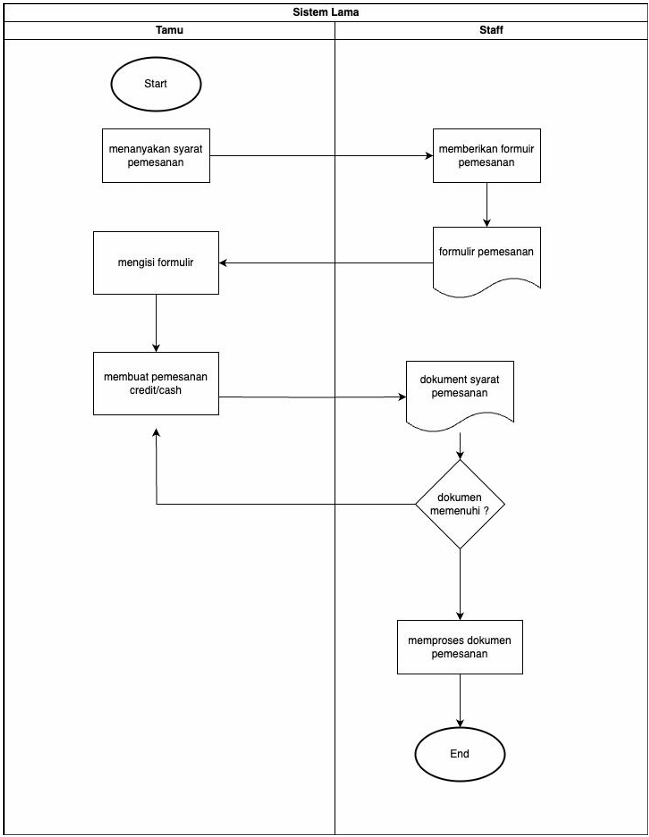
\includegraphics[width=0.90\linewidth]{Analisa sistem yang sedang berjalan.png}
    \caption{Analisa Sistem Yang Sedang Berjalan}
\end{figure}
% -----------------------------------------------------------------------------%
\section{Analisa Sistem Yang Diusulkan}
% -----------------------------------------------------------------------------%
\par Berdasarkan hasil analisa sistem yang sedang berjalan, proses seperti itu membuat proses pemesanan berjalan lama, dan sulit ditangani jika terdapat lebih dari 1 pemesan dalam satu waktu. Oleh karena itu, dibutuhkanlah sebuah sistem yang dapat digunakan oleh pengelola Perumahan Kamela permai dalam menangani proses pemesanan yang terkomputerisasi, dengan membuat sebuah sistem pemesanan berbasis web. Dimana proses pemesanan hanya dilakukan menggunaan smartphone/laptop.
\par Dalam Sistem  sudah terdapat panduan bagaimana dan apa syarat untuk memesan sebuah ruman di Perumahan Kamela Permai. Data calon  akan langsung tersimpan didalam sistem sehingga pengelola hanya perlu mengunggu data tersebut masuk berapa pun banyaknya.
\par Adapun analisa sistem yang diusulkan penulis dapat dilihat pada Gambar 4.2 berikut:
\begin{figure}
\centering
    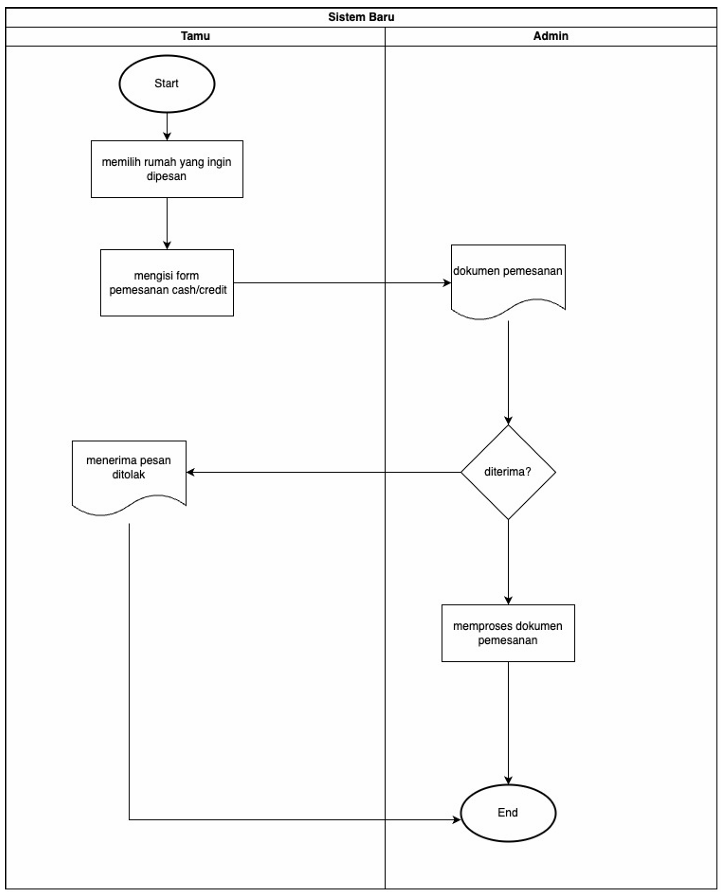
\includegraphics[width=0.90\linewidth]{Analisa Sistem Yang Diusulkan.png}
    \caption{Analisa Sistem Yang Diusulkan}
\end{figure}
% -----------------------------------------------------------------------------%
\subsection{Rencana Sistem Usulan}
% -----------------------------------------------------------------------------%
\subsection{\textit{Use Case Diagram}}
% -----------------------------------------------------------------------------%
\par Use Case Diagram terdiri dari \textit{Actor, Use Case} dan serta hubungannya. \textit{Use Case Diagram} adalah sesuatu yang penting untuk memvisualisasikan, menspesifikasikan dan mendokumentasikan kebutuhan perilaku sistem. \textit{Use Case Diagram} digunakan untuk menjelaskan kegiatan apa saja yang dapat dilakukan oleh \textit{user} pada sistem yang sedang berjalan. Penggambaran sistem dalam bentuk \textit{use case} dapat dilihat pada Gambar 4.3 berikut:
\begin{figure}
    \centering
    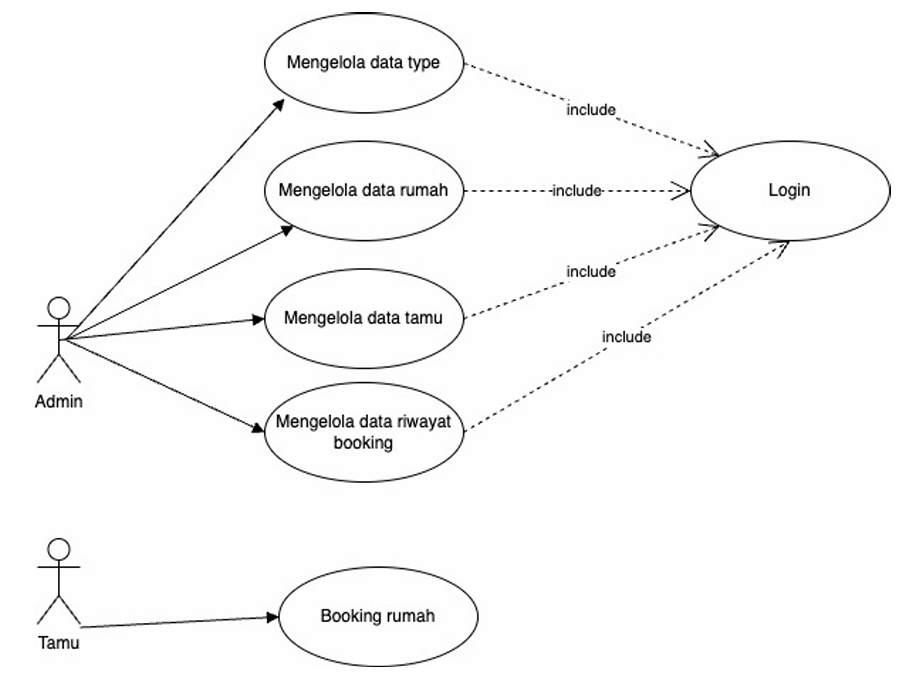
\includegraphics[width=1.0\linewidth]{Use Case Diagram.png}
    \caption{\textit{Use Case Diagram}}
    \label{fig:enter-label}
\end{figure}


    \par Adapun penjelasan mengenai aktor-aktor pada use case diagram sistem yang usulan ini dapat dilihat pada tabel berikut:

\begin{longtable}[c]{|l|l|p{9cm}|} % Gunakan p{10cm} agar teks panjang dibungkus
\captionsetup{position=above} % Menempatkan caption di atas tabel
\caption{Deskripsi Aktor}
\label{tab:my-table}\\
\hline
Aktor & Sinonim          & Deskripsi                                                                                                                                                                                      \\ \hline
\endfirsthead
% Kosongkan untuk menghilangkan teks "continued from previous page"
\endhead
%
Admin  & \textit{Administrator}             & Orang / Bagian yang bertugas mengelola data tamu, rumah type rumah didalam sistem.                                      \\ \hline
Tamu  & \textit{Guest}     & Tamu adalah calon pelanggan yang bisa merupakan siapa saja dan dapat memesan perumahan di Perumahan Kamela Permai.                                                                                                                   \\ \hline
\end{longtable}

\par Berikut ini merupakan deskripsi dari masing-masing \textit{use case} yang berada pada Sistem Informasi Pemesanan Perumahan Kamela Permai.
\begin{longtable}[c]{|l|l|p{9cm}|} % Gunakan p{10cm} agar teks panjang dibungkus
\captionsetup{position=above} % Menempatkan caption di atas tabel
\caption{Deskripsi \textit{Use Case} Diagram}
\label{tab:my-table}\\
\hline
No & \textit{Use Case}          & Deskripsi                                                                                                                                                                                      \\ \hline
\endfirsthead
% Kosongkan untuk menghilangkan teks "continued from previous page"
\endhead
%
1  & Login             & \textit{Use Case} ini menggambarkan aktor masuk ke sistem dengan menggunakan \textit{username} dan \textit{password}.                                      \\ \hline
2  & Kelola Data Rumah     & \textit{Use Case} ini menggambarkan admin dapat mengelola data, antara lain; mengubah status dan mengedit blok dan nomor rumah.                                                                                                                   \\ \hline
3  & Kelola Data Tamu         & \textit{Use Case} ini menggambarkan admin dapat mengubah status, melihat data yang diinputkan tamu serte menghapus data tamu.                                                                            \\ \hline
4  & Kelola Data riwayat    & \textit{Use Case} ini menggambarkan admin dapat mengelola data Riwayat Tamu yang berhasil memesan rumah lewat sistem.               \\ \hline
5  & Booking    & \textit{Use Case} ini menggambarkan tamu dapat memesan dengan memilih salah satu rumah dan memanginputkan data yang diperlukan. \\ \hline
\end{longtable}

\begin{enumerate}
    \item Skenario\textit{ Use Case Diagram}
\par Skenario \textit{use case} menyatakan urutan pesan dan tindakan tunggal yang ada pada sistem. Berikut ditampilkan skenario use case dari setiap use case yang telah ada.
\end{enumerate}
\begin{enumerate}[label=\alph*.]
    \item Skenario \textit{Use Case Login}
	\par Skenario \textit{Use Case Login} dapat dilihat pada tabel berikut:

        \begin{longtable}{|p{5cm}|p{9cm}|}
	    \caption{Skenario \textit{Use Case Login}}
	    \label{tab:my-table} \\ \hline
	    \multicolumn{1}{|c|}{\textbf{Komponen}} & \multicolumn{1}{c|}{\textbf{Deskripsi}} \\ \hline
	    \endfirsthead
	    \hline
	    \multicolumn{1}{|c|}{\textbf{Komponen}} & \multicolumn{1}{c|}{\textbf{Deskripsi}} \\ \hline
	    \endhead
	    Nama \textit{Use Case} & \textit{Login} \\ \hline
	    Deskripsi & \textit{Use case} ini menggambarkan \textit{actor} masuk ke sistem dengan menggunakan \textit{username} dan \textit{password}. \\ \hline
	    Aktor & Admin \\ \hline
	    \textit{Pre-Condition} & Sistem menampilkan halaman \textit{login}. \\ \hline
	    \textit{Post-Condition} & Aktor berhasil \textit{login}. \\ \hline
	    \multicolumn{2}{|c|}{\textbf{Skenario Normal}} \\ \hline
	    \multicolumn{1}{|c|}{\textbf{Aksi Aktor}} & \multicolumn{1}{c|}{\textbf{Reaksi Sistem}} \\ \hline
	    1. Aktor melakukan \textit{login} dengan menginput \textit{username} dan \textit{password} & \\ \hline
	    & 2. Sistem melakukan verifikasi \textit{login}. \\ \hline
	    & 3. Sistem menampilkan \textit{form} menu utama. \\ \hline
	    \multicolumn{2}{|c|}{\textbf{Skenario Gagal}} \\ \hline
	    \multicolumn{1}{|c|}{\textbf{Aksi Aktor}} & \multicolumn{1}{c|}{\textbf{Reaksi Sistem}} \\ \hline
	    1. Aktor melakukan \textit{login} dengan menginput \textit{username} dan \textit{password} & \\ \hline
	    & 2. Sistem melakukan verifikasi \textit{login}. \\ \hline
	    & 3. Sistem menampilkan pesan gagal login karena kredensial tidak valid. \\ \hline
	\end{longtable}


    
    \item Skenario \textit{Use Case} Kelola Data Rumah
	\par Skenario \textit{Use Case} Kelola Data Rumah dapat dilihat pada tabel berikut:

       \begin{longtable}{|p{5cm}|p{9cm}|}
	    \caption{Skenario \textit{Use Case} Kelola Data Rumah}
	    \label{tab:my-table} \\ \hline
	    \multicolumn{1}{|c|}{\textbf{Komponen}} & \multicolumn{1}{c|}{\textbf{Deskripsi}} \\ \hline
	    \endfirsthead
	    \endhead
	    Nama \textit{Use Case} & Kelola Data Rumah \\ \hline
	    Deskripsi & \textit{Use case} ini menggambarkan actor dapat mengubah data rumah \\ \hline
	    Aktor & Admin \\ \hline
	    \textit{Pre-Condition} & Sistem memasuki halaman data rumah. \\ \hline
	    \textit{Post-Condition} & Sistem menampilkan halaman data rumah. \\ \hline
	    \multicolumn{2}{|c|}{\textbf{Skenario Normal}} \\ \hline
	    \multicolumn{1}{|c|}{\textbf{Aksi Aktor}} & \multicolumn{1}{c|}{\textbf{Reaksi Sistem}} \\ \hline
	    1. Aktor masuk ke halaman data rumah & \\ \hline
	    & 2. Sistem menampilkan halaman data rumah \\ \hline
	    3. Aktor melihat, mengubah nomor/blok dan status rumah & \\ \hline
	    & 4. Sistem menyimpan perubahan data rumah \\ \hline
	    \multicolumn{2}{|c|}{\textbf{Skenario Alternatif: Gagal}} \\ \hline
	    \multicolumn{1}{|c|}{\textbf{Aksi Aktor}} & \multicolumn{1}{c|}{\textbf{Reaksi Sistem}} \\ \hline
	    1. Admin menuju halaman keuangan & \\ \hline
	    & 2. Sistem menampilkan halaman data pegawai \\ \hline
	    3. Aktor melihat, mengubah nomor/blok dan status rumah & \\ \hline
	    & 4. Sistem menampilkan pesan gagal menyimpan penambahan atau perubahan data rumah \\ \hline
	\end{longtable}

        
    \item Skenario \textit{Use Case} Kelola Data Tamu
	\par Skenario \textit{Use Case} Kelola Data Tamu dapat dilihat pada tabel berikut:

    \begin{longtable}{|p{5cm}|p{9cm}|}
	    \caption{Skenario \textit{Use Case} Kelola Data Tamu}
	    \label{tab:my-table} \\ \hline
	    \multicolumn{1}{|c|}{\textbf{Komponen}} & \multicolumn{1}{c|}{\textbf{Deskripsi}} \\ \hline
	    \endfirsthead
	    \endhead
	    Nama \textit{Use Case} & Kelola Data Tamu \\ \hline
	    Deskripsi & \textit{Use case} ini menggambarkan aktor dapat mengelola data tamu antara lain; menerima pesanan tamu dan menghapus tamu \\ \hline
	    Aktor & Admin \\ \hline
	    \textit{Pre-Condition} & Sistem memasuki halaman tamu. \\ \hline
	    \textit{Post-Condition} & Sistem menampilkan halaman tamu. \\ \hline
	    \multicolumn{2}{|c|}{\textbf{Skenario Normal}} \\ \hline
	    \multicolumn{1}{|c|}{\textbf{Aksi Aktor}} & \multicolumn{1}{c|}{\textbf{Reaksi Sistem}} \\ \hline
	    1. Aktor masuk ke halaman tamu & \\ \hline
	    & 2. Sistem menampilkan halaman data tamu \\ \hline
	    3. Aktor melihat, mengubah dan menghapus data tamu & \\ \hline
	    & 4. Sistem mengubah atau menghapus data tamu \\ \hline
	    \multicolumn{2}{|c|}{\textbf{Skenario Alternatif: Gagal}} \\ \hline
	    \multicolumn{1}{|c|}{\textbf{Aksi Aktor}} & \multicolumn{1}{c|}{\textbf{Reaksi Sistem}} \\ \hline
	    1. Aktor masuk ke halaman data jabatan & \\ \hline
	    & 2. Sistem menampilkan halaman data jabatan \\ \hline
	    3. Aktor melihat, mengubah, dan menghapus data tamu & \\ \hline
	    & 4. Sistem menampilkan pesan gagal menyimpan pengubahan atau penghapusan data tamu \\ \hline
	\end{longtable}
     
    
    \item Skenario \textit{Use Case Booking}
    
	\par Skenario \textit{Use Case Booking} dapat dilihat pada tabel berikut:

        \begin{longtable}{|p{5cm}|p{9cm}|}
	    \caption{Skenario \textit{Use Case} Booking}
	    \label{tab:my-table} \\ \hline
	    \multicolumn{1}{|c|}{\textbf{Komponen}} & \multicolumn{1}{c|}{\textbf{Deskripsi}} \\ \hline
	    \endfirsthead
	    \endhead
	    Nama \textit{Use Case} & Booking \\ \hline
	    Deskripsi & \textit{Use case} ini menggambarkan aktor dapat membuat pemesanan rumah. \\ \hline
	    Aktor & Tamu \\ \hline
	    \textit{Pre-Condition} & Sistem memasuki halaman \textit{siteplan}. \\ \hline
	    \textit{Post-Condition} & Sistem menampilkan halaman \textit{siteplan}. \\ \hline
	    \multicolumn{2}{|c|}{\textbf{Skenario Normal}} \\ \hline
	    \multicolumn{1}{|c|}{\textbf{Aksi Aktor}} & \multicolumn{1}{c|}{\textbf{Reaksi Sistem}} \\ \hline
	    1. Aktor masuk ke halaman \textit{siteplan} & \\ \hline
	    & 2. Sistem menampilkan \textit{siteplan} \\ \hline
	    3. Aktor melihat dan memilih rumah untuk dipesan & \\ \hline
	    & 4. Sistem menampilkan opsi metode kredit atau tunai \\ \hline
	    5. Aktor memilih metode & \\ \hline
	    & 6. Sistem memberikan halaman formulir untuk pemesanan \\ \hline
	    7. Aktor mengisi formulir & \\ \hline
	    & 8. Sistem menyimpan data dan memberikan pesan berhasil \\ \hline
	    \multicolumn{2}{|c|}{\textbf{Skenario Alternatif: Gagal}} \\ \hline
	    \multicolumn{1}{|c|}{\textbf{Aksi Aktor}} & \multicolumn{1}{c|}{\textbf{Reaksi Sistem}} \\ \hline
	    1. Aktor memilih rumah yang telah dipesan oleh orang lain & \\ \hline
	    & 2. Sistem menampilkan pesan gagal karena rumah tidak tersedia \\ \hline
	    3. Aktor mencoba mengisi formulir dengan data yang tidak valid & \\ \hline
	    & 4. Sistem menampilkan pesan gagal menyimpan data pemesanan \\ \hline
	\end{longtable}
    
    
    \item Skenario \textit{Use Case} Kelola \textit{Type}

\par Skenario \textit{Use Case} Kelola \textit{Type} dapat dilihat pada tabel berikut.
        
        \begin{longtable}{|p{5cm}|p{9cm}|}
	    \captionsetup{position=above} % Menempatkan caption di atas tabel
	    \caption{Skenario \textit{Use Case} Kelola Data Tamu}
	    \label{tab:my-table} \\ \hline
	    \multicolumn{1}{|c|}{\textbf{Komponen}} & \multicolumn{1}{c|}{\textbf{Deskripsi}} \\ \hline
	    \endfirsthead
	    \endhead
	    Nama \textit{Use Case} & Kelola \textit{Type} \\ \hline
	    Deskripsi & \textit{Use case} ini menggambarkan aktor dapat menambah atau menghapus gambar serta mengganti harga untuk tiap \textit{Type}. \\ \hline
	    Aktor & Admin \\ \hline
	    \textit{Pre-Condition} & Sistem memasuki halaman data \textit{Type}. \\ \hline
	    \textit{Post-Condition} & Sistem menampilkan halaman data \textit{Type}. \\ \hline
	    \multicolumn{2}{|c|}{\textbf{Skenario Normal}} \\ \hline
	    \multicolumn{1}{|c|}{\textbf{Aksi Aktor}} & \multicolumn{1}{c|}{\textbf{Reaksi Sistem}} \\ \hline
	    1. Aktor masuk ke halaman data \textit{Type} & \\ \hline
	    & 2. Sistem menampilkan halaman data \textit{Type} \\ \hline
	    3. Aktor melihat, menambah, mengubah, dan menghapus data \textit{Type} & \\ \hline
	    & 4. Sistem menyimpan penambahan, pengubahan, atau pengapusan data \textit{Type} \\ \hline
	    \multicolumn{2}{|c|}{\textbf{Skenario Alternatif: Gagal}} \\ \hline
	    \multicolumn{1}{|c|}{\textbf{Aksi Aktor}} & \multicolumn{1}{c|}{\textbf{Reaksi Sistem}} \\ \hline
	    1. Aktor masuk ke halaman data type & \\ \hline
	    & 2. Sistem menampilkan halaman data \textit{Type} \\ \hline
	    3. Aktor melihat, menambah, mengubah dan menghapus data \textit{Type} & \\ \hline
	    & 4. Sistem menampilkan pesan gagal menyimpan penambahan, pengubahan atau pengapusan data \textit{Type} \\ \hline
	\end{longtable}
  
        
    \item Skenario \textit{Use Case} Kelola Data Riwayat
	
	\par Skenario \textit{Use Case} Kelola Riwayat dapat dilihat pada tabel berikut.

        \begin{longtable}{|p{5cm}|p{9cm}|}
	    \captionsetup{position=above} % Menempatkan caption di atas tabel
	    \caption{Skenario \textit{Use Case} Kelola Data Riwayat}
	    \label{tab:my-table} \\ \hline
	    \multicolumn{1}{|c|}{\textbf{Komponen}} & \multicolumn{1}{c|}{\textbf{Deskripsi}} \\ \hline
	    \endfirsthead
	    \endhead
	    Nama \textit{Use Case} & Kelola Data Riwayat \\ \hline
	    Deskripsi & \textit{Use case} ini menggambarkan aktor dapat melihat atau menghapus data riwayat pemesanan yang berhasil. \\ \hline
	    Aktor & Admin \\ \hline
	    Kondisi Awal & Sistem memasuki halaman data riwayat \\ \hline
	    Kondisi Akhir & Sistem menampilkan halaman data riwayat \\ \hline
	    \multicolumn{2}{|c|}{\textbf{Skenario Normal}} \\ \hline
	    \multicolumn{1}{|c|}{\textbf{Aksi Aktor}} & \multicolumn{1}{c|}{\textbf{Reaksi Sistem}} \\ \hline
	    1. Aktor masuk ke halaman data riwayat & \\ \hline
	    & 2. Sistem menampilkan halaman data riwayat \\ \hline
	    3. Aktor melihat dan menghapus data riwayat & \\ \hline
	    & 4. Sistem menghapus data riwayat \\ \hline
	    \multicolumn{2}{|c|}{\textbf{Skenario Alternatif: Gagal}} \\ \hline
	    \multicolumn{1}{|c|}{\textbf{Aksi Aktor}} & \multicolumn{1}{c|}{\textbf{Reaksi Sistem}} \\ \hline
	    1. Aktor masuk ke halaman data riwayat & \\ \hline
	    & 2. Sistem menampilkan halaman data riwayat \\ \hline
	    3. Aktor melihat, menambah, mengubah dan menghapus data \textit{type} & \\ \hline
	    & 4. Sistem menampilkan pesan gagal penghapusan data \textit{type}, kesalahan sistem pada \textit{database}. \\ \hline
	\end{longtable}

    
\end{enumerate}
% -----------------------------------------------------------------------------%
\subsection{\textit{Activity Diagram}}
% -----------------------------------------------------------------------------%
\par Diagram aktivitas menggambarkan aliran fungsionalitas sistem yang dapat digunakan untuk menunjukkan aliran kejadian \textit{(Flow of events)} dalam \textit{use case}. Setiap proses yang terjadi dalam sistem akan digambarkan secara rinci dan lengkap, dengan langkah demi langkahnya mulai dari masukan hingga keluaran.
\par Proses sistem Pemesanan Rumah di Perumahan Kamela Permai yang diusulkan ini akan dijelaskan pada Activity Diagram berikut:

\begin{enumerate}
    \item \textit{Activity Diagram Login}
        \par \textit{Activity Diagram Login } dapat dilihat dari gambar berikut:
            \begin{figure}
                \centering
                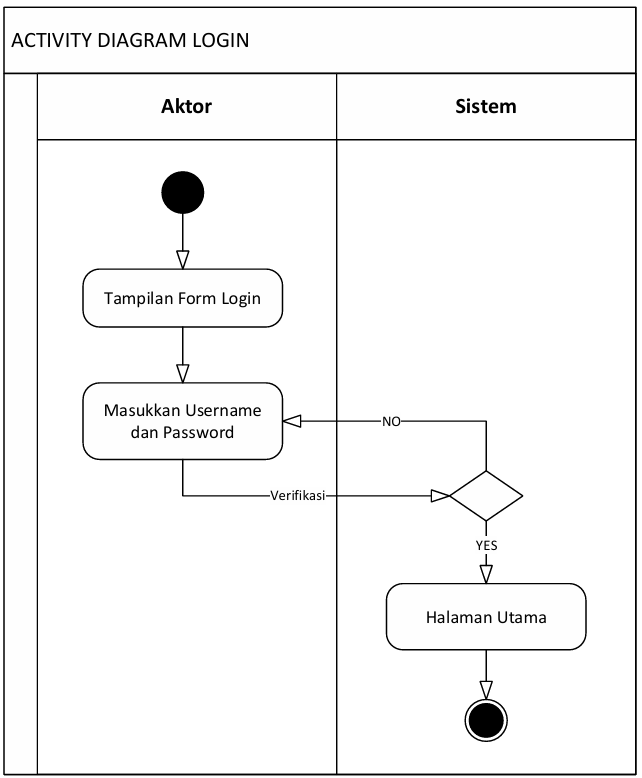
\includegraphics[width=0.95\linewidth]{uml/Activity Diagram - Login.png}
                \caption{\textit{Activity Diagram} Login}
                \label{fig:enter-label}
            \end{figure}
            
    \item \textit{Activity Diagram} Kelola Rumah
        \par \textit{Activity Diagram} Kelola Rumah dapat dilihat dari gambar berikut:
            \begin{figure}
                \centering
                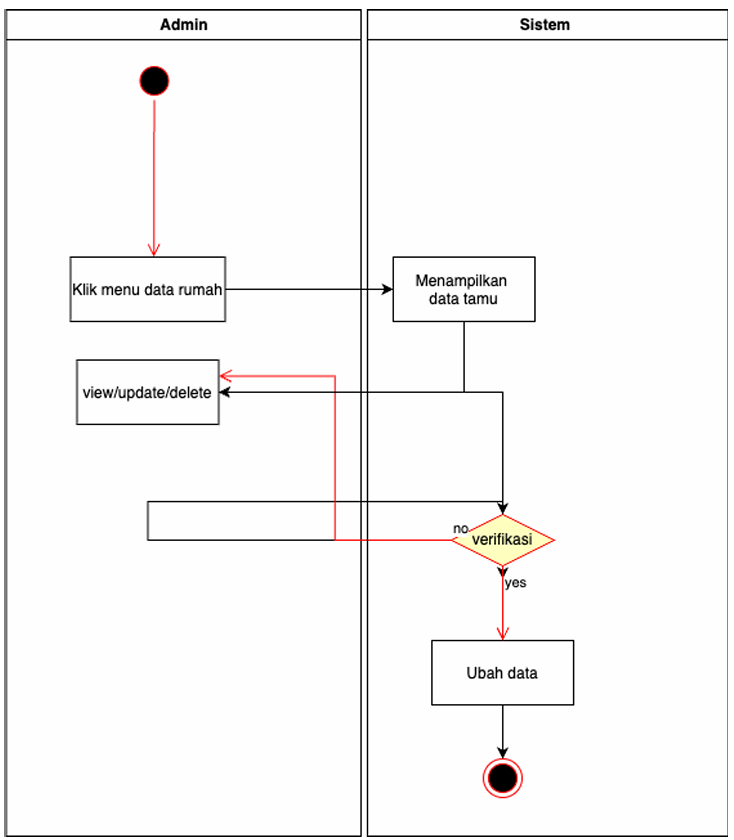
\includegraphics[width=0.95\linewidth]{uml/Activity Diagram - Kelola Rumah.png}
                \caption{\textit{Activity Diagram} Kelola Rumah}
                \label{fig:enter-label}
            \end{figure}
	
	\item \textit{Activity Diagram} Kelola Data Tamu
        \par \textit{Activity Diagram} Kelola Data Tamu dapat dilihat dari gambar berikut:
            \begin{figure}
                \centering
                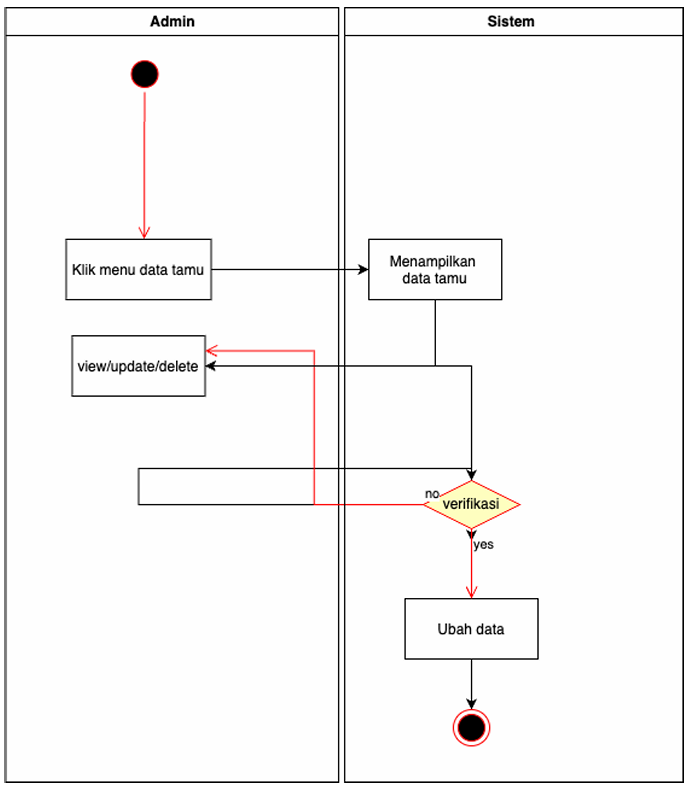
\includegraphics[width=0.95\linewidth]{uml/Activity Diagram - Kelola Tamu.png}
                \caption{\textit{Activity Diagram} Kelola Data Tamu}
            \end{figure}

    \item \textit{Activity Diagram} Kelola Data \textit{Type}
        \par \textit{Activity Diagram} Kelola Data \textit{Type} dapat dilihat dari gambar berikut:
            \begin{figure}
                \centering
                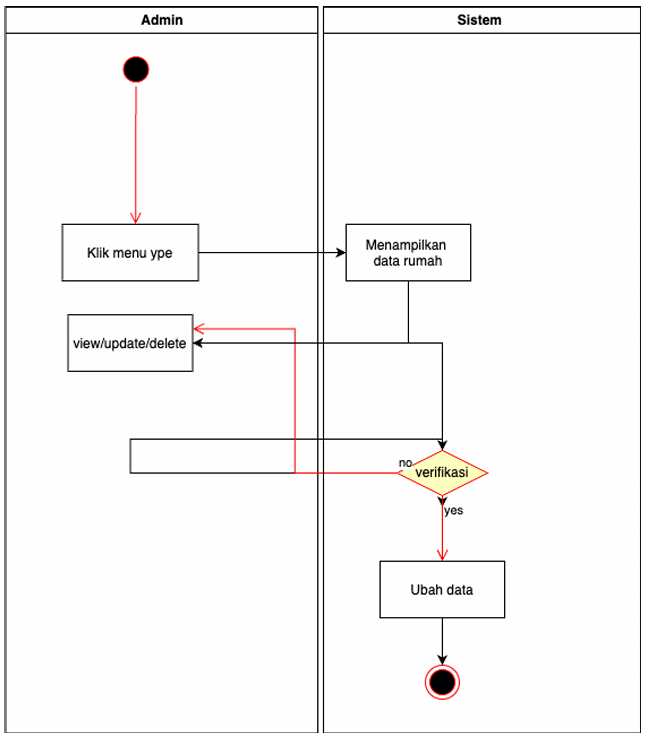
\includegraphics[width=0.95\linewidth]{uml/Activity Diagram - Kelola Type.png}
                \caption{\textit{Activity Diagram} Kelola Data \textit{Type}}
                \label{fig:enter-label}
            \end{figure}
    \item \textit{Activity Diagram Booking}
        \par \textit{Activity Diagram Booking} dapat dilihat dari gambar berikut:
            \begin{figure}
                \centering
                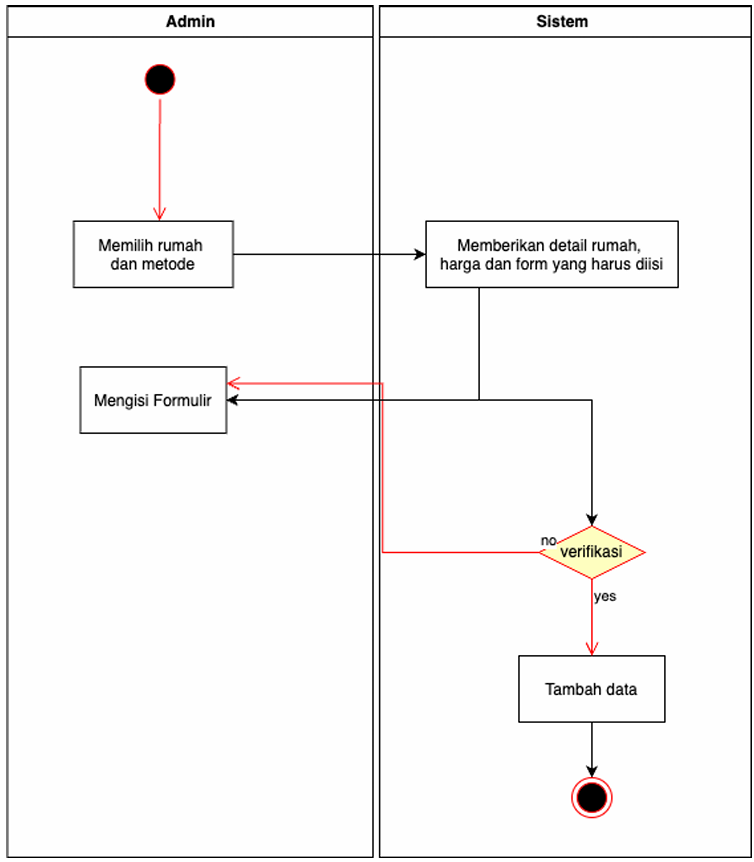
\includegraphics[width=0.95\linewidth]{uml/Activity Diagram - Booking.png}
                \caption{\textit{Activity Diagram Booking}}
                \label{fig:enter-label}
            \end{figure}
\end{enumerate}

% -----------------------------------------------------------------------------%
\subsection{\textit{Class Diagram}}
% -----------------------------------------------------------------------------%
\par \textit{Class Diagram} amerupakan diagram yang menunjukkan beberapa \textit{class} yang ada pada sistem serta hubungannya secara logic. \textit{Class Diagram} yang dibuat pada tahap design ini, merupakan deskripsi lengkap dari \textit{class-class} yang ditangani oleh sistem, dimana masing-masing \textit{class} telah dilengkapi dengan atribut dan operasi-operasi yang diperlukan.
\par Adapun \textit{Class Diagram} pada sistem yang diusulkan ini dapat dilihat pada gambar berikut:

\begin{figure}
    \centering
    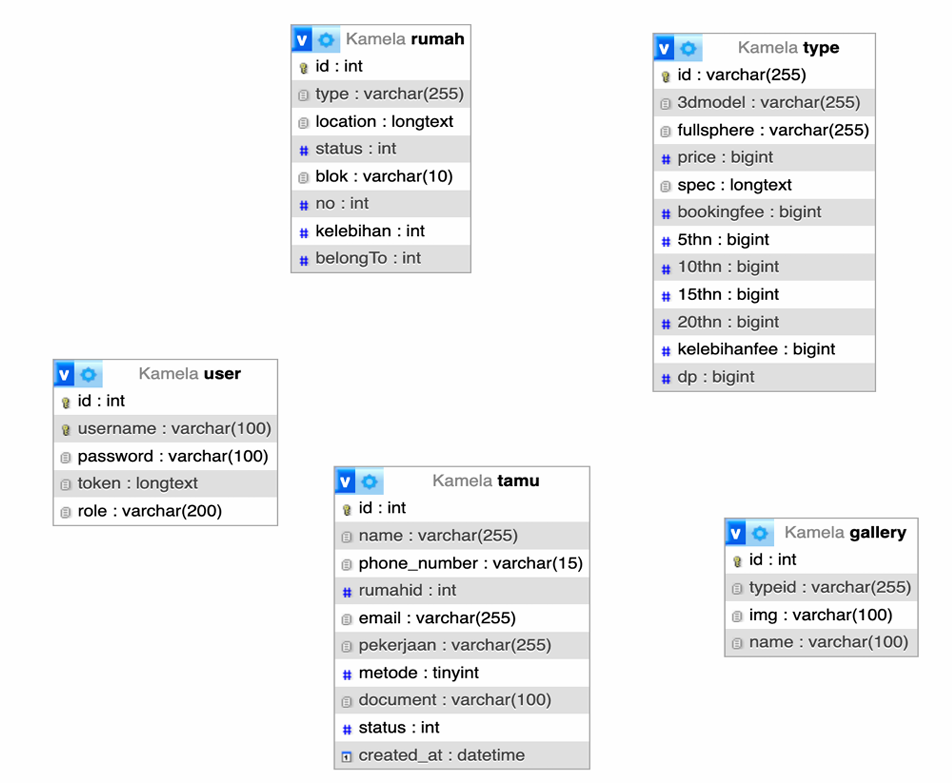
\includegraphics[width=0.95\linewidth]{Class Diagram.png}
    \caption{\textit{Class Diagram}}
\end{figure}

% -----------------------------------------------------------------------------%
\subsection{Perancangan \textit{Database}}
% -----------------------------------------------------------------------------%
\par Pada perancangan \textit{database} terdapat beberapa tabel yang saling berelasi. Perancangan \textit{database} yang akan digunakan pada sistem, didasari oleh data instansi. Perancangan ini bertujuan agar field data yang memiliki relasi dapat terhubung pada tabel di \textit{database}, sehingga proses pengaksesan data akan terorganisir dengan lebih baik.

\par Berikut adalah detail perancangan serta relasi yang ada pada \textit{database} sistem informasi pemesanan perumahan:

\begin{enumerate}
    \item \textbf{Tabel Absen}
    
    \begin{itemize}
        \item Nama Tabel: Users
        \item \textit{Primary Key}: id
    \end{itemize}

   \begin{longtable}{|p{3cm}|p{3cm}|p{2cm}|p{3cm}|}
	    \captionsetup{position=above} % Menempatkan caption di atas tabel
	    \caption{Tabel Struktur Database User}
	    \label{tab:struktur-database} \\ \hline
	    \multicolumn{1}{|c|}{\textbf{Nama Field}} & \multicolumn{1}{c|}{\textbf{Type}} & \multicolumn{1}{c|}{\textbf{Null}} & \multicolumn{1}{c|}{\textbf{Default}} \\ \hline
	    \endfirsthead
	    \hline
	    \multicolumn{1}{|c|}{\textbf{Nama Field}} & \multicolumn{1}{c|}{\textbf{Type}} & \multicolumn{1}{c|}{\textbf{Null}} & \multicolumn{1}{c|}{\textbf{Default}} \\ \hline
	    \endhead
	    id & int(11) & No & \\ \hline
	    username & varchar(255) & No & \\ \hline
	    password & varchar(255) & No & \\ \hline
	    token & varchar(255) & Yes & \\ \hline
	    role & varchar(255) & No & \\ \hline
	\end{longtable}


    \item \textbf{Tabel Type}

    \begin{itemize}
        \item Nama Tabel: Type
        \item \textit{Primary Key}: id
    \end{itemize}

     \begin{longtable}{|p{3cm}|p{3cm}|p{2cm}|p{3cm}|}
	    \captionsetup{position=above} % Menempatkan caption di atas tabel
	    \caption{Tabel Struktur Type}
	    \label{tab:struktur-database} \\ \hline
	    \multicolumn{1}{|c|}{\textbf{Column}} & \multicolumn{1}{c|}{\textbf{Type}} & \multicolumn{1}{c|}{\textbf{Null}} & \multicolumn{1}{c|}{\textbf{Default}} \\ \hline
	    \endfirsthead
	    \hline
	    \multicolumn{1}{|c|}{\textbf{Column}} & \multicolumn{1}{c|}{\textbf{Type}} & \multicolumn{1}{c|}{\textbf{Null}} & \multicolumn{1}{c|}{\textbf{Default}} \\ \hline
	    \endhead
	    id & varchar(255) & No & \\ \hline
	    3dmodel & varchar(255) & No & \\ \hline
	    price & bigInt & No & \\ \hline
	    spec & json & No & \\ \hline
	    bookingfee & bigInt & No & \\ \hline
		dp & bigInt & No & \\ \hline
		5thn & bigInt & Yes & \\ \hline
		10thn & bigInt & Yes & \\ \hline
		15thn & bigInt & Yes & \\ \hline
		20thn & bigInt & Yes & \\ \hline
		additionalfee & bigInt & Yes & \\ \hline
	\end{longtable}

    \item \textbf{Tabel House}
    
    \begin{itemize}
        \item Nama Tabel: house
        \item \textit{Primary Key}: id
    \end{itemize}
    
    \begin{longtable}{|p{3cm}|p{3cm}|p{2cm}|p{3cm}|}
	    \captionsetup{position=above} % Menempatkan caption di atas tabel
	    \caption{Tabel Struktur House}
	    \label{tab:struktur-database} \\ \hline
	    \multicolumn{1}{|c|}{\textbf{Column}} & \multicolumn{1}{c|}{\textbf{Type}} & \multicolumn{1}{c|}{\textbf{Null}} & \multicolumn{1}{c|}{\textbf{Default}} \\ \hline
	    \endfirsthead
	    \hline
	    \multicolumn{1}{|c|}{\textbf{Column}} & \multicolumn{1}{c|}{\textbf{Type}} & \multicolumn{1}{c|}{\textbf{Null}} & \multicolumn{1}{c|}{\textbf{Default}} \\ \hline
	    \endhead
	    id & int(11) & No & \\ \hline
	    type & varchar(255) & No & \\ \hline
	    location & varchar(255) & No & \\ \hline
	    status & int(3) & Yes & \\ \hline
	    blok & varchar(255) & No & \\ \hline
		no & int(3) & No & \\ \hline
		additional & int(255) & Yes & \\ \hline
		belongTo & int(11) & Yes & \\ \hline
	\end{longtable}

    \item \textbf{Tabel Guest}
    
    \begin{itemize}
        \item Nama Tabel: guest
        \item \textit{Primary Key}: id
    \end{itemize}

   \begin{longtable}{|p{3cm}|p{3cm}|p{2cm}|p{3cm}|}
	    \captionsetup{position=above} % Menempatkan caption di atas tabel
	    \caption{Tabel Guest}
	    \label{tab:struktur-database} \\ \hline
	    \multicolumn{1}{|c|}{\textbf{Column}} & \multicolumn{1}{c|}{\textbf{Type}} & \multicolumn{1}{c|}{\textbf{Null}} & \multicolumn{1}{c|}{\textbf{Default}} \\ \hline
	    \endfirsthead
	    \hline
	    \multicolumn{1}{|c|}{\textbf{Column}} & \multicolumn{1}{c|}{\textbf{Type}} & \multicolumn{1}{c|}{\textbf{Null}} & \multicolumn{1}{c|}{\textbf{Default}} \\ \hline
	    \endhead
	    id & int(11) & No & \\ \hline
	    name & varchar(50) & No & \\ \hline
	    phone\_number &	varchar(15) & No & \\ \hline
	    house\_id & int(11) & No & \\ \hline
	    email & varchar(50) & No & \\ \hline
		job & varchar(50) & No & \\ \hline
		method & tinyInt & No & \\ \hline
		document & varchar(50) & No & \\ \hline
		status & int(11) & No & \\ \hline
		created\_at & date & No & current\_datetime \\ \hline
	\end{longtable}

    \item \textbf{Tabel Gallery}
    
    \begin{itemize}
        \item Nama Tabel: Gallery
        \item \textit{Primary Key}: id
    \end{itemize}

    \begin{longtable}{|p{3cm}|p{3cm}|p{2cm}|p{3cm}|}
	    \captionsetup{position=above} % Menempatkan caption di atas tabel
	    \caption{Tabel Struktur Database Gallery}
	    \label{tab:struktur-database} \\ \hline
	    \multicolumn{1}{|c|}{\textbf{Nama Field}} & \multicolumn{1}{c|}{\textbf{Type}} & \multicolumn{1}{c|}{\textbf{Null}} & \multicolumn{1}{c|}{\textbf{Default}} \\ \hline
	    \endfirsthead
	    \hline
	    \multicolumn{1}{|c|}{\textbf{Nama Field}} & \multicolumn{1}{c|}{\textbf{Type}} & \multicolumn{1}{c|}{\textbf{Null}} & \multicolumn{1}{c|}{\textbf{Default}} \\ \hline
	    \endhead
	    id & int(11) & No & \\ \hline
	    typeid & varchar(11) & No & \\ \hline
	    name & varchar(255) & Yes & \\ \hline
	    image & varchar(255) & No & \\ \hline
	\end{longtable}

\end{enumerate}
% -----------------------------------------------------------------------------%
\subsection{Perancangan\textit{ Interface}}
% -----------------------------------------------------------------------------%
\par Perancangan antarmuka pengguna merupakan suatu proses yang kompleks, hal ini didasari karena antarmuka pengguna merupakan bagian dari sistem yang akan dikendalikan oleh pengguna dan merupakan tahap persiapan untuk rancang bangun implementasi. Oleh karena itu, untuk mendapatkan sistem yang dapat berjalan sesuai dengan fungsi yang diharapkan, diperlukannya pengalaman dalam merancang antarmuka pengguna, kreativitas yang tinggi, analisis tugas dan dapat menyesuaikan dengan kebutuhan serta kemampuan pengguna.

    \begin{enumerate}
        \item Perancangan \textit{Homepage Interface Landing Page}
        \par Pada halaman landing page ini, yang merupakan tampilan awal sistem yang berguna untuk memberikan informasi dasar mengenai fitur sistem Pemesanan Rumah di Perumahan Kamela Permai. Pengguna dapat melakukan login dan mengakses informasi lebih lanjut melalui menu "pesan sekarang".
        \begin{figure}
            \centering
            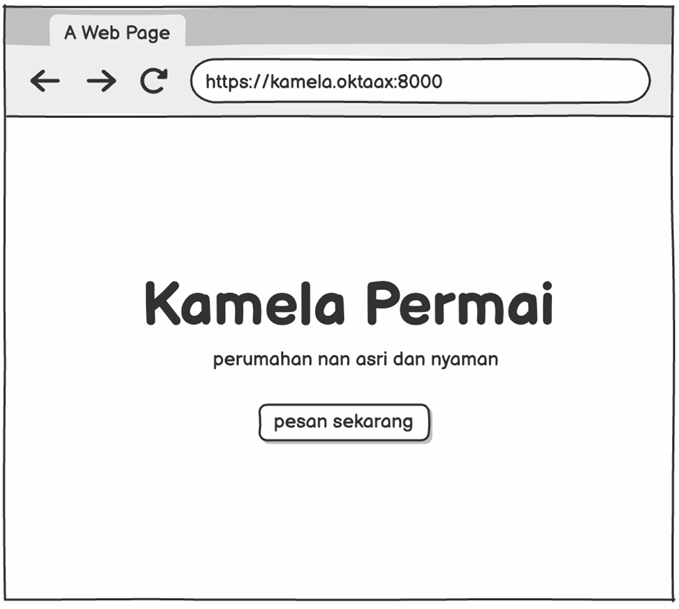
\includegraphics[width=0.75\linewidth]{Wireframe/Landing Page.png}
            \caption{Perancangan \textit{Interface Home}}
        \end{figure}
        
        \item Perancangan \textit{Interface Login}
        \par Perancangan \textit{interface Login} berguna untuk mengakses Sistem Presensi Karyawan yang terdiri dari \textit{Username, password} dan \textit{Login}.
        \begin{figure}
            \centering
            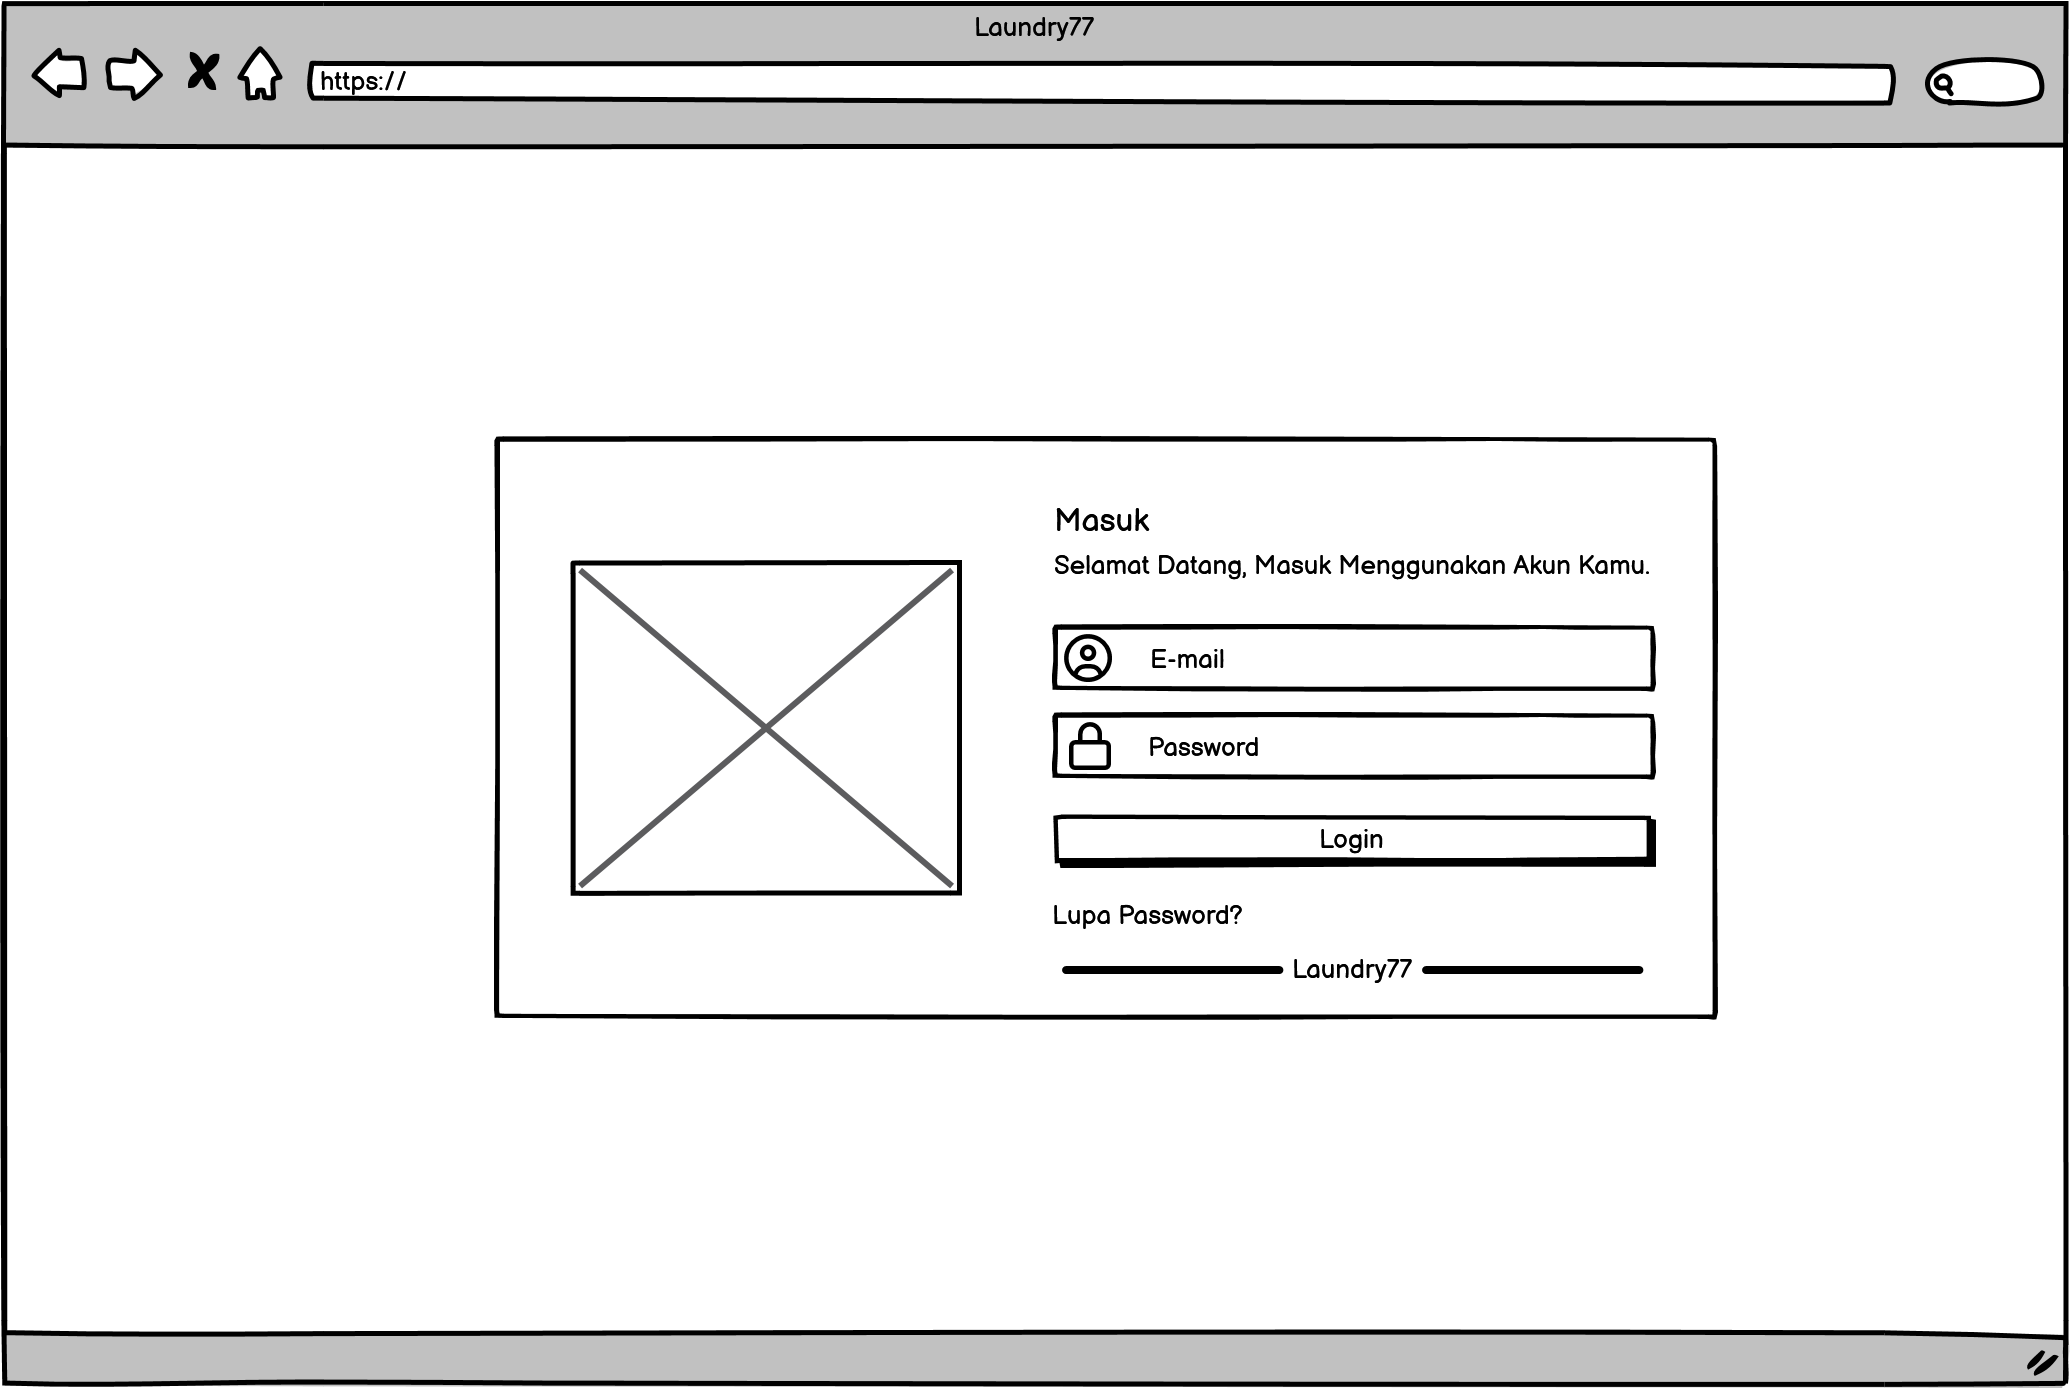
\includegraphics[width=0.75\linewidth]{Wireframe/Login.png}
            \caption{Perancangan \textit{Interface Login}}
        \end{figure}
        
        \item Perancangan \textit{Interface Dashboard}
        \par Berikut perancangan Interface Dashboard dapat dilihat pada gambar berikut.
        \begin{figure}
            \centering
            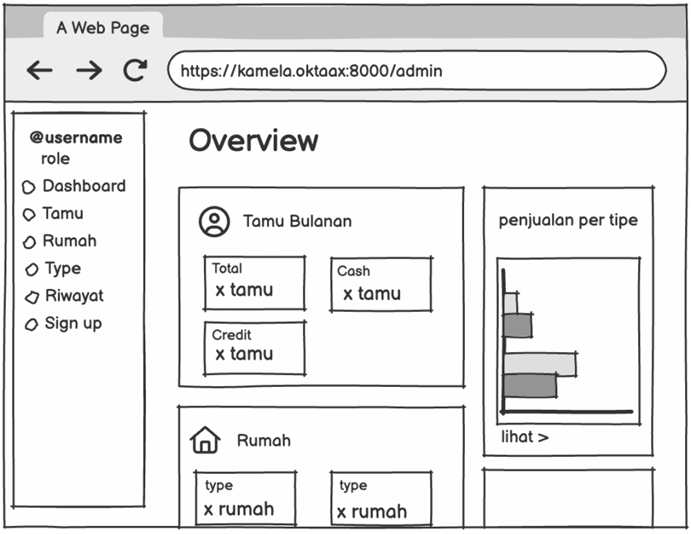
\includegraphics[width=0.75\linewidth]{Wireframe/Dashboard.png}
            \caption{Perancangan \textit{Interface Dashboard}}
        \end{figure}
        
        \item Perancangan \textit{Interface Data Rumah}
        \par Berikut perancangan \textit{Interface Data Rumah} dapat dilihat pada gambar berikut.
        \begin{figure}
            \centering
            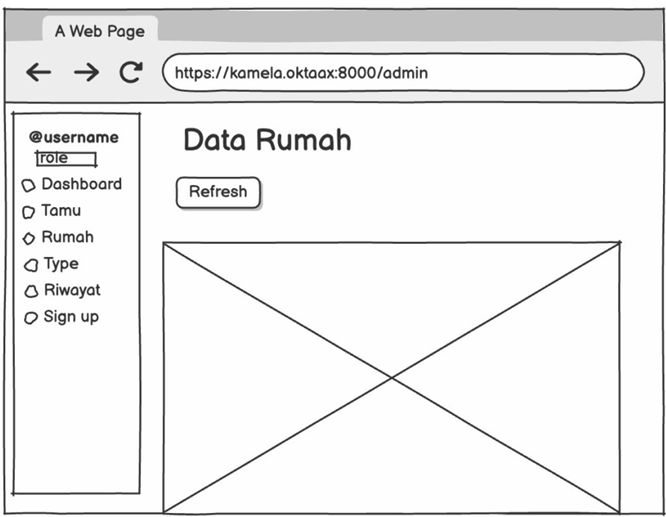
\includegraphics[width=0.75\linewidth]{Wireframe/Data Rumah.png}
            \caption{Perancangan \textit{Interface Data Rumah}}
        \end{figure}
        
        \item Perancangan \textit{Interface} Data Tamu
        \par Berikut adalah perancangan \textit{Interface} Data Tamu.
        \begin{figure}
            \centering
            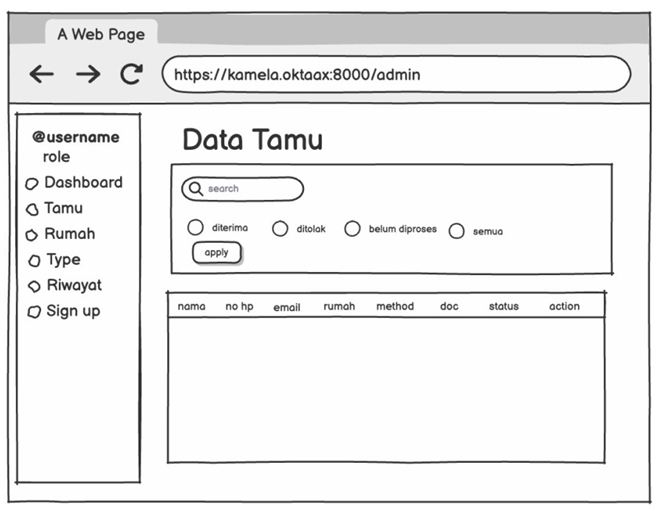
\includegraphics[width=0.75\linewidth]{Wireframe/Data Tamu.png}
            \caption{Perancangan \textit{Interface} Data Tamu}
        \end{figure}
        
        \item Perancangan \textit{Interface} Data Riwayat Pemesanan
        \par Berikut adalah perancangan \textit{Interface} Data Riwayat Pemesanan.
        \begin{figure}
            \centering
            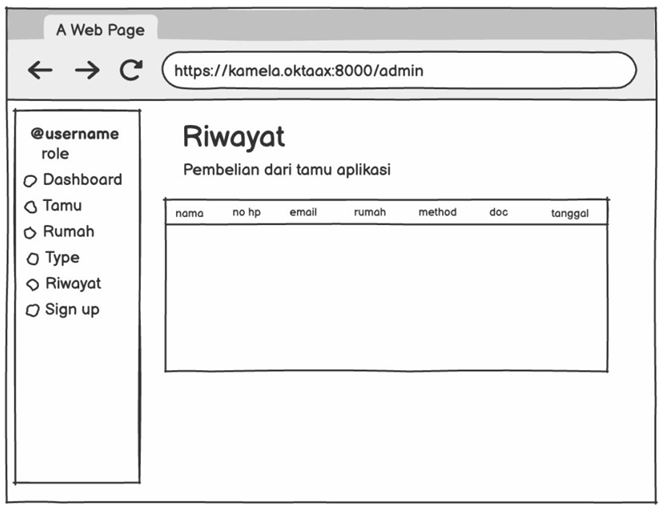
\includegraphics[width=0.75\linewidth]{Wireframe/Riwayat Pemesanan.png}
            \caption{Perancangan \textit{Interface} Data Riwayat Pemesanan}
        \end{figure}
        
        \item Perancangan \textit{Interface} Data Type
        \par Berikut adalah perancangan \textit{Interface} Data Type.
        \begin{figure}
            \centering
            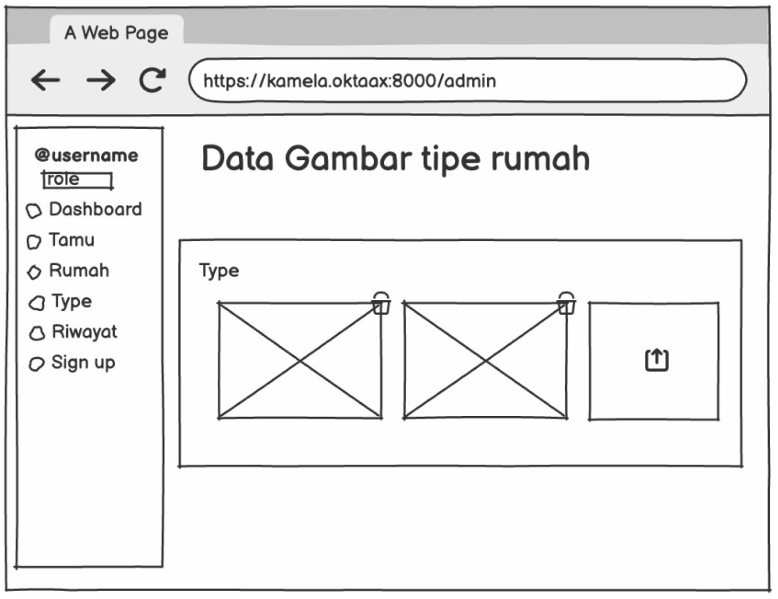
\includegraphics[width=0.75\linewidth]{Wireframe/Data Tipe.png}
            \caption{Perancangan \textit{Interface} Data Type}
        \end{figure}
        
        \item Perancangan \textit{Interface} Harga
        \par Berikut adalah perancangan \textit{Interface} Harga.
        \begin{figure}
            \centering
            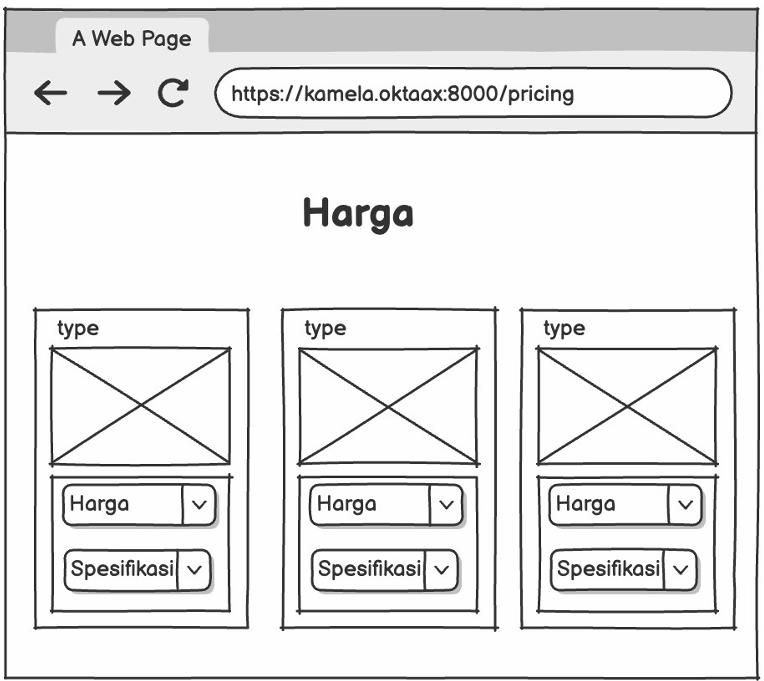
\includegraphics[width=0.75\linewidth]{Wireframe/Harga.png}
            \caption{Perancangan \textit{Interface} Harga}
        \end{figure}
        
        \item Perancangan \textit{Interface} Halaman Gallery
        \par Berikut adalah perancangan \textit{Interface} Halaman Gallery.
        \begin{figure}
            \centering
            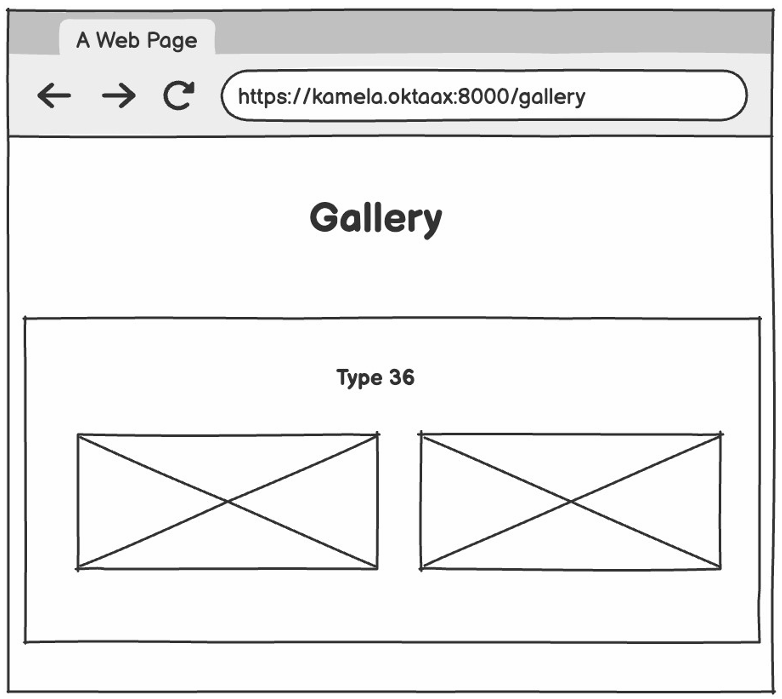
\includegraphics[width=0.75\linewidth]{Wireframe/Gallery.png}
            \caption{Perancangan \textit{Interface} Halaman Gallery}
        \end{figure}
        
        \item Perancangan \textit{Interface} Panduan
        \par Berikut adalah perancangan \textit{Interface} Panduan.
        \begin{figure}
            \centering
            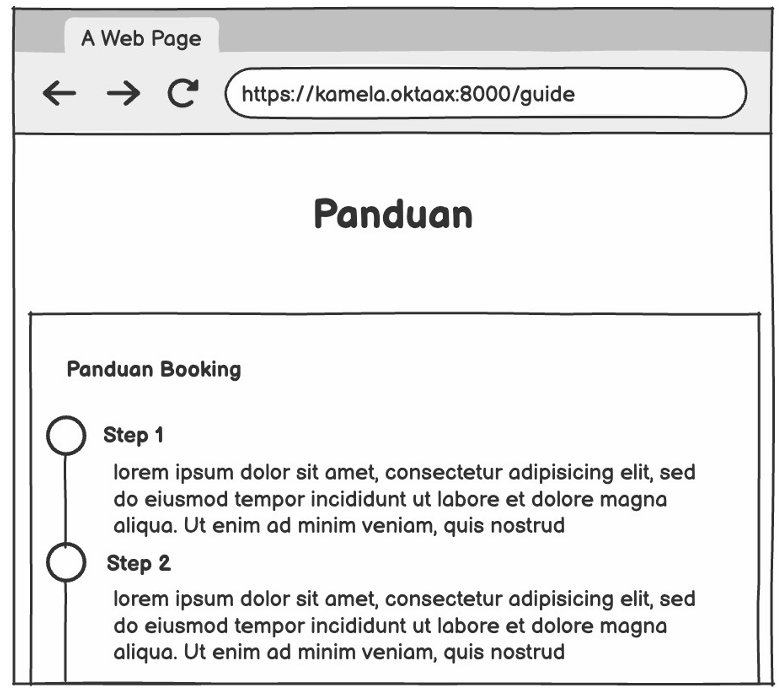
\includegraphics[width=0.72\linewidth]{Wireframe/Panduan.png}
            \caption{Perancangan \textit{Interface} Panduan}
        \end{figure}
        
        \item Perancangan \textit{Interface Site Plan}
        \par Berikut adalah perancangan \textit{Interface Site Plan}.
        \begin{figure}
            \centering
            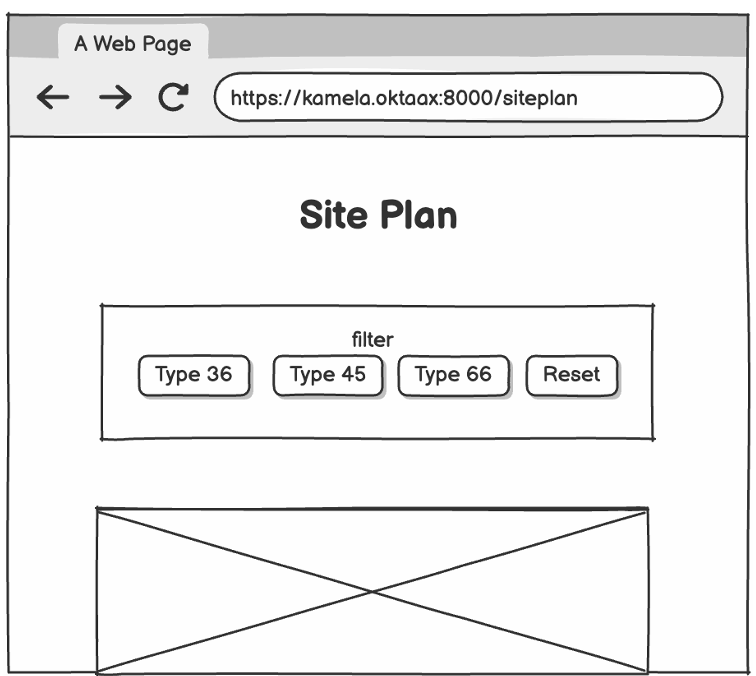
\includegraphics[width=0.72\linewidth]{Wireframe/Site Plan.png}
            \caption{Perancangan \textit{Interface Site Plan.}}
        \end{figure}

    \end{enumerate}
% -----------------------------------------------------------------------------%
\section{Hasil}

\subsection{Implementasi Sitem}
\par Implementasi sistem merupakan bentuk asli sistem yang dibuat berdasarkan rancangan interface yang telah dibuat sebelumnya, sehingga akan menampilkan bentuk sistem secara keseluruhannya. Tahap implementasi merupakan tahap meletakkan sistem supaya siap untuk dioperasikan, tahap ini termasuk juga kegiatan menulis kode program jika tidak digunakan paket perangkat lunak aplikasi dan pengetesan program. Berikut adalah beberapa hasil implementasi sistem.

\begin{enumerate}
    \item Halaman \textit{Home}
    \par Tampilan halaman home  dapat dilihat pada gambar berikut:

    \begin{figure}
        \centering
        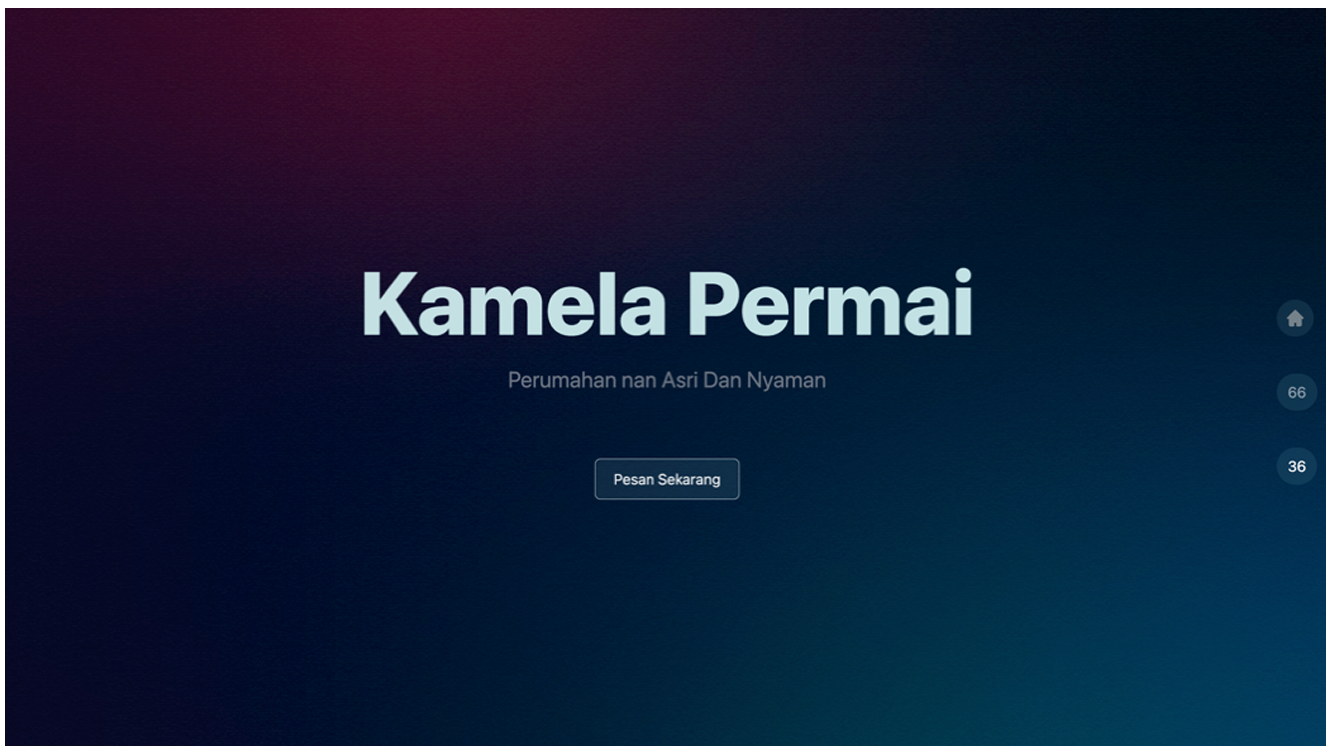
\includegraphics[width=0.75\linewidth]{Implementasi/Home.png}
        \caption{Halaman \textit{Home}}
    \end{figure}
    
    \item Halaman \textit{Login}
    \par Berikut adalah tampilan login, untuk megakses sistem penggua diharuskan mengisi \textit{username} dan \textit{password} terlebih dahulu dapat dilihat pada gambar berikut.
    \begin{figure}
        \centering
        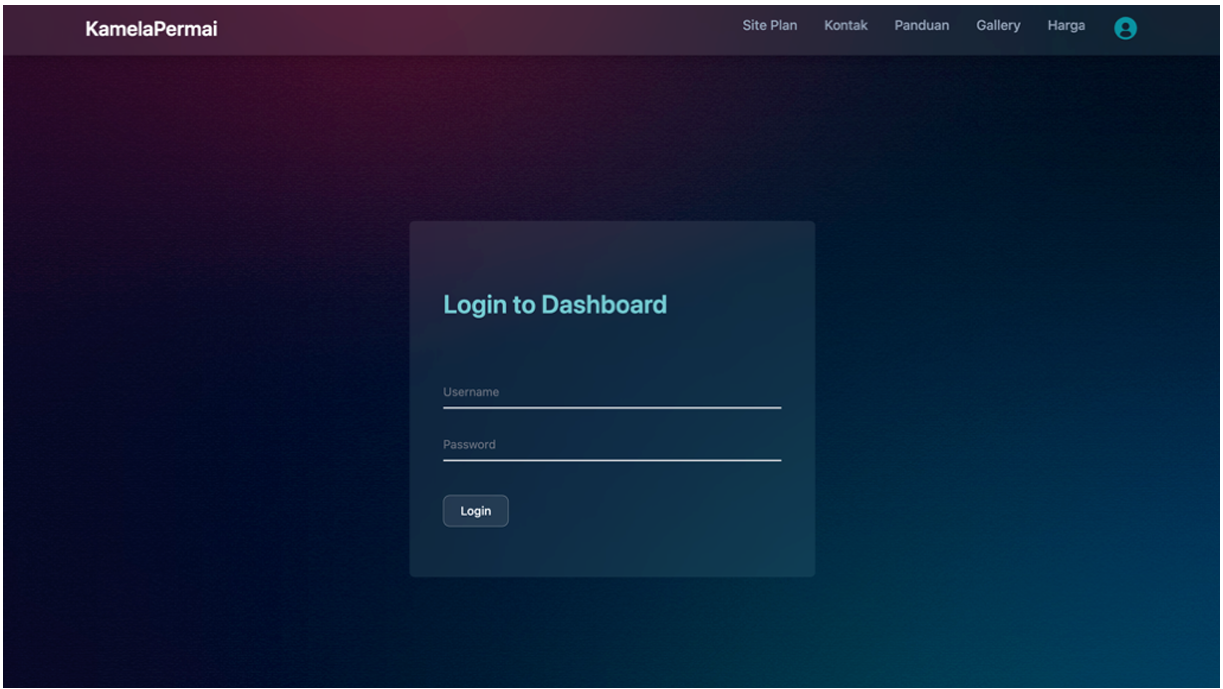
\includegraphics[width=0.75\linewidth]{Implementasi/Login.png}
        \caption{Halaman \textit{Login}}
    \end{figure}
    
    \item Halaman Dashboard Admin
    \par Berikut halaman dashboard yang menampilkan beberapa fitur yang tersedia pada sistem dapat dilihat pada gambar berikut.
    \begin{figure}
        \centering
        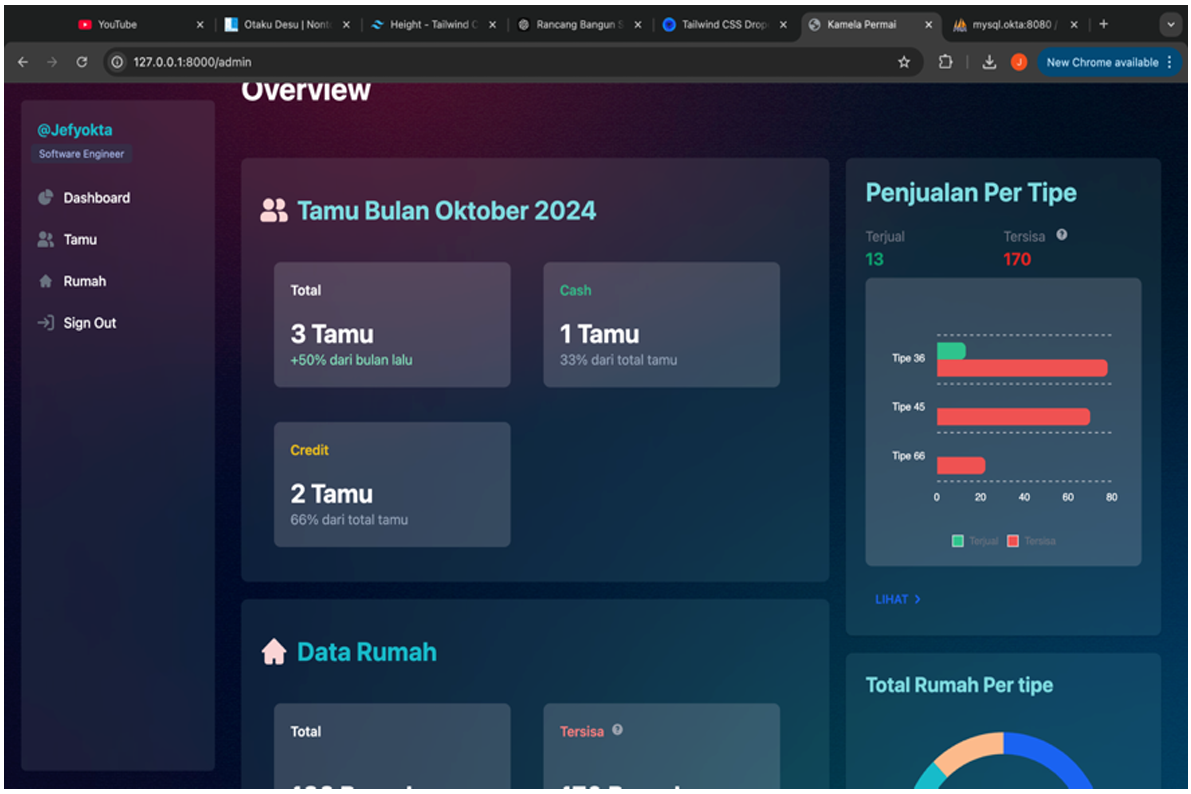
\includegraphics[width=0.75\linewidth]{Implementasi/Dashboard Admin.png}
        \caption{Halaman Dashboard Admin}
    \end{figure}
    
    \item Halaman Data Rumah
    \par Pada gambar dibawah merupakan gambar halaman untuk melakukan pengubahan pada data rumah serta mengubah status ketersediaanya yang dapat dilihat pada gambar berikut.
    \begin{figure}
        \centering
        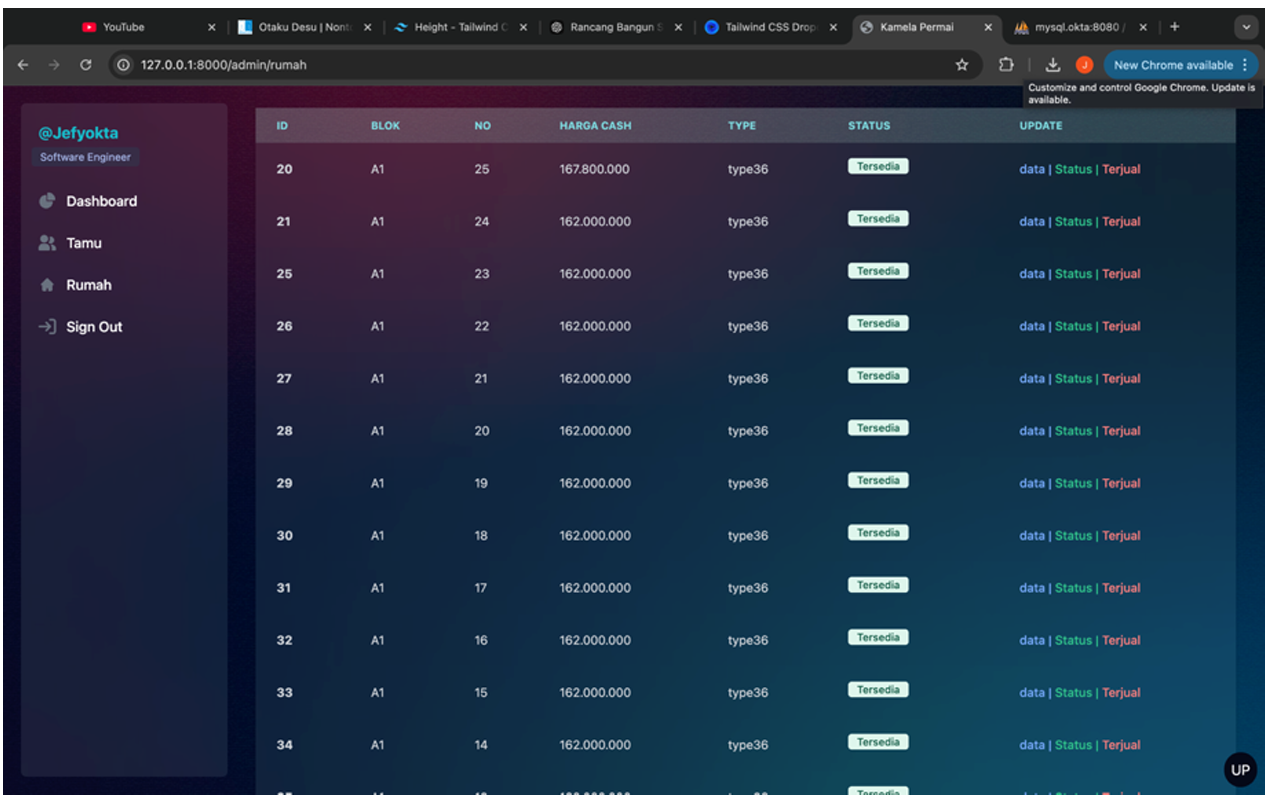
\includegraphics[width=0.75\linewidth]{Implementasi/Data Rumah.png}
        \caption{Halaman Data Rumah}
    \end{figure}

	 \begin{figure}
	        \centering
	        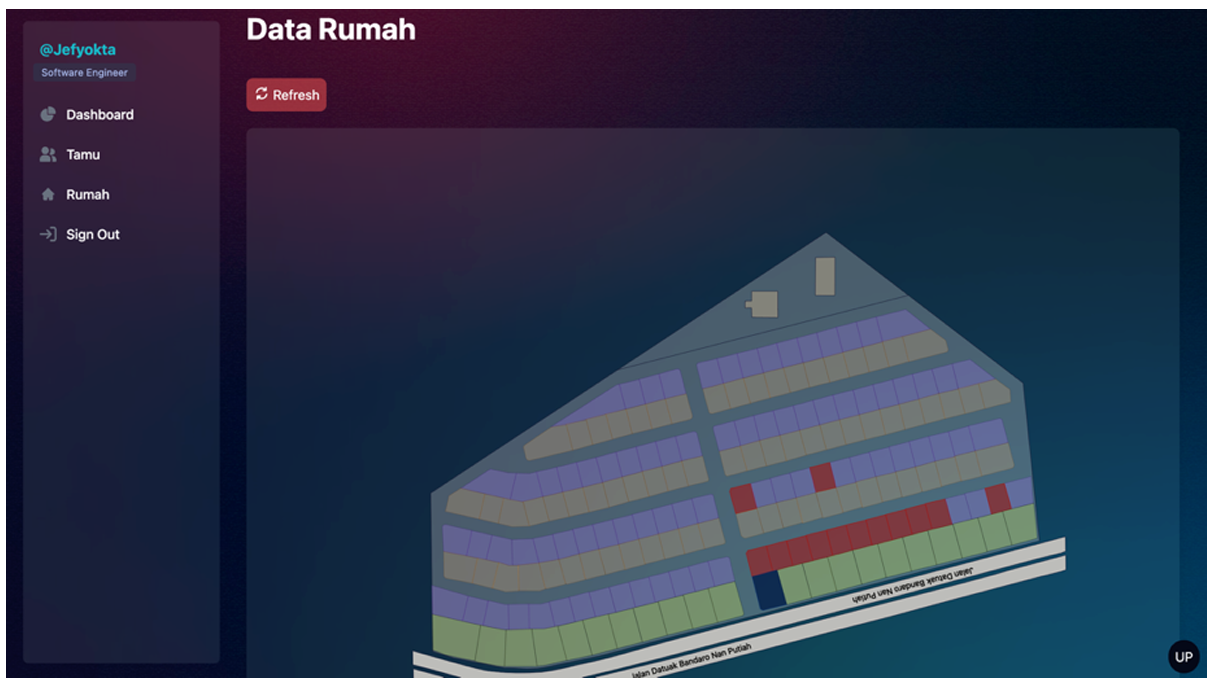
\includegraphics[width=0.75\linewidth]{Implementasi/Data Rumah 2.png}
	        \caption{Halaman Data Rumah 2}
	    \end{figure}
    
    \item Halaman Data Tamu
    \par Pada halaman data tamu ini terdapat no, nama, nomor telepon, email, dokumen dan aksi. Pada halaman ini admin dapat menerima pemesanan atau menghapusnya dapat dilihat pada gambar berikut.
    \begin{figure}
        \centering
        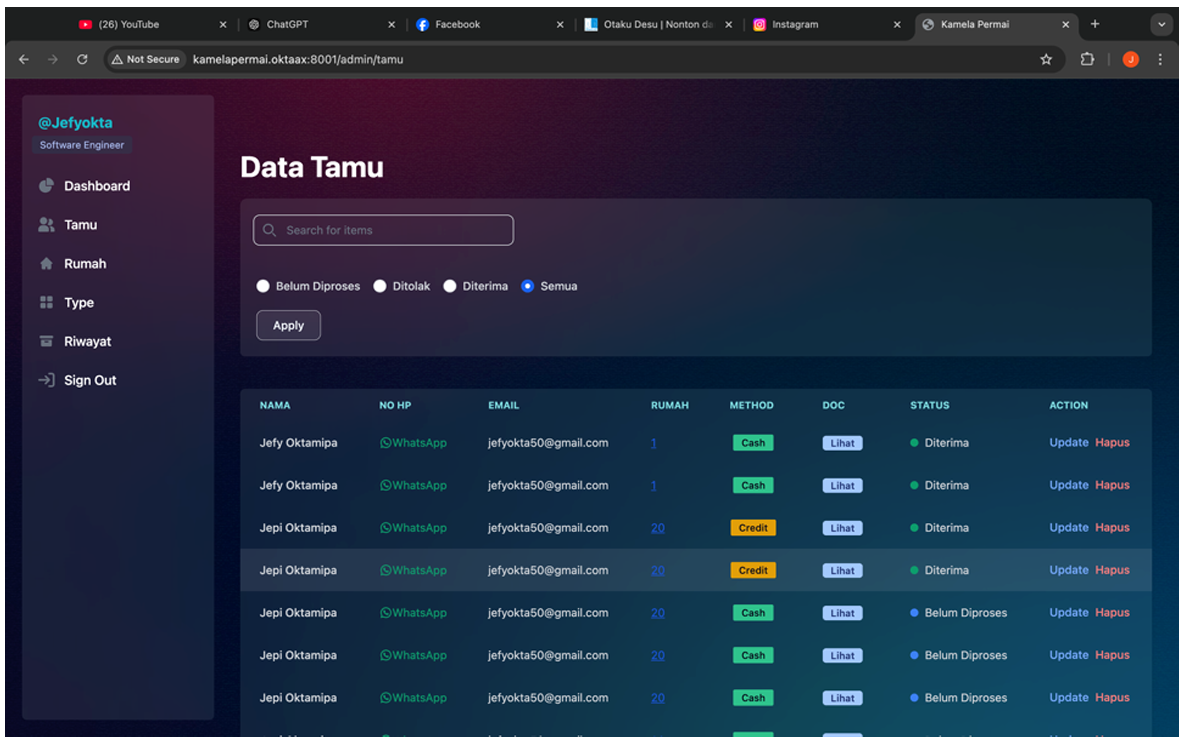
\includegraphics[width=0.75\linewidth]{Implementasi/Data Tamu.png}
        \caption{Halaman Data Tamu}
    \end{figure}
    
    \item Halaman Data Riwayat Pemesanan
    \par Pada halaman data riwayat terdapat data tamu yang berhasil booking. Admin dapat melihatnya seperti digambar berikut.
    \begin{figure}
        \centering
        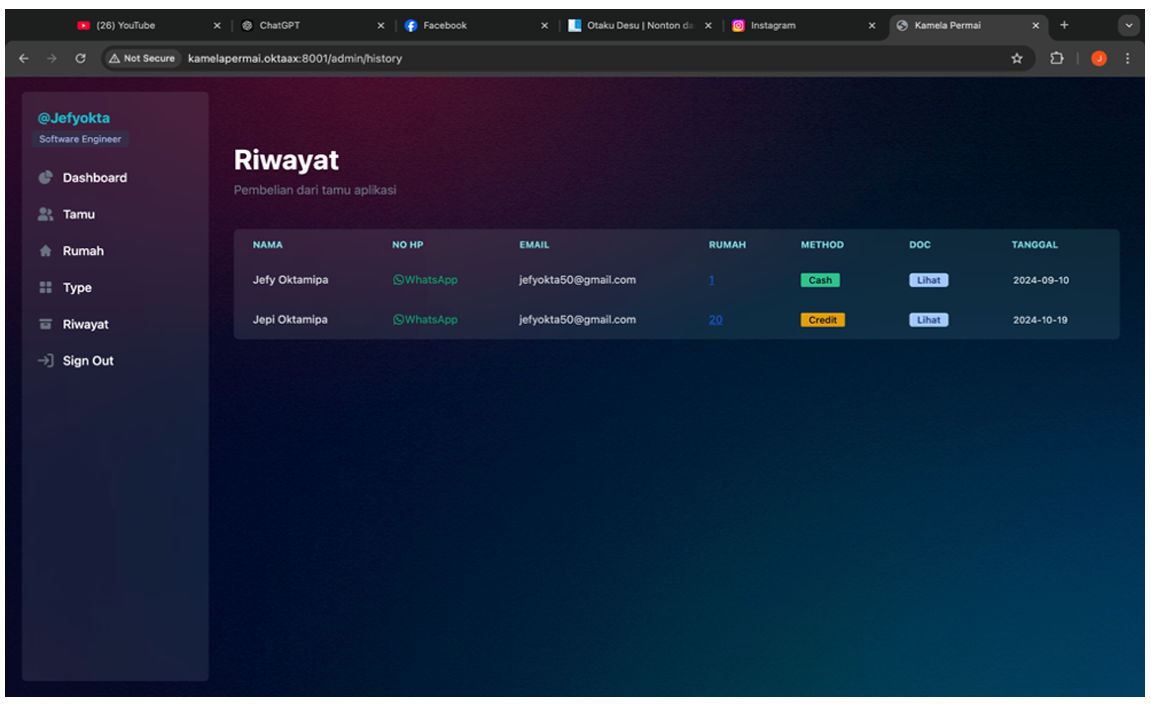
\includegraphics[width=0.75\linewidth]{Implementasi/Data Riwayat Pemesanan.png}
        \caption{Halaman Data Riwayat Pemesanan}
    \end{figure}
    
    \item Halaman Data \textit{Type}
    \par Pada halaman data \textit{Type} Terdapat gambar untuk setiap tipe yang dapat di tambah ataupun dihapus oleh admin. Dapat dilihat pada gambar berikut:.
    \begin{figure}
        \centering
        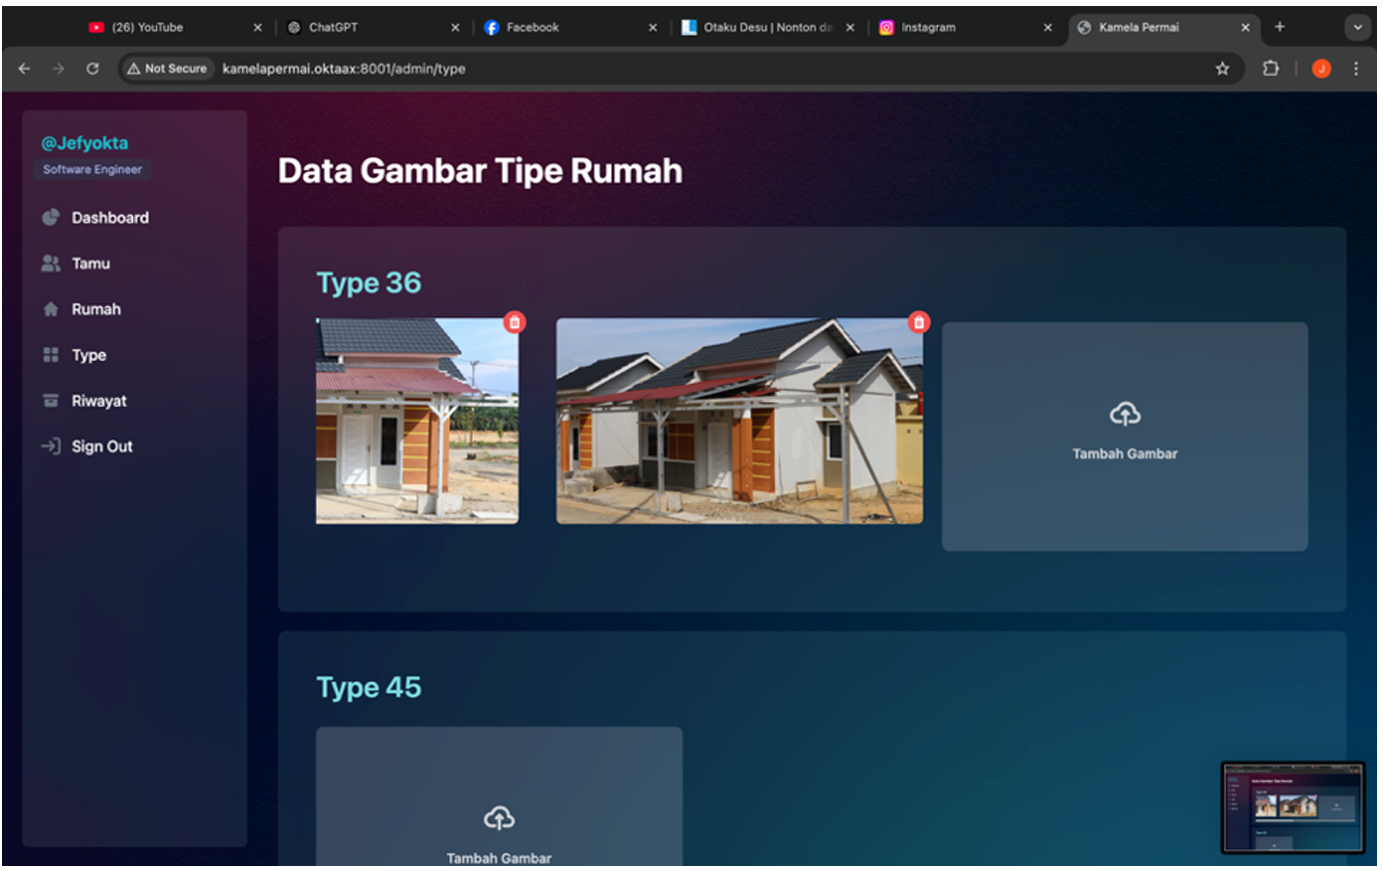
\includegraphics[width=0.75\linewidth]{Implementasi/Data Type.png}
        \caption{Halaman Data \textit{Type}}
    \end{figure}
    
    \item Halaman Harga
    \par Pada halaman harga terdapat harga cash, booking, cicilian dan spesifikasi setiap type nya yang dapat dilihat pada gambar berikut.
    \begin{figure}
        \centering
        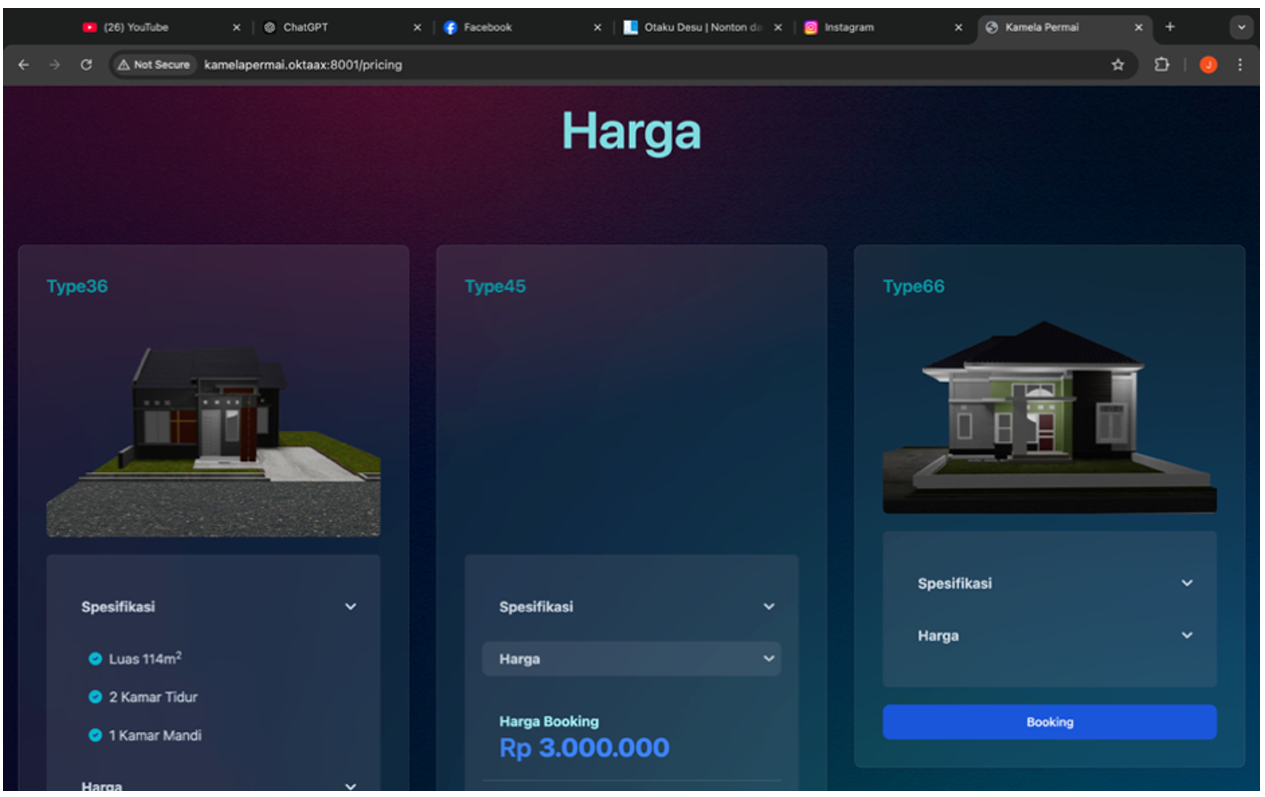
\includegraphics[width=0.75\linewidth]{Implementasi/Harga.png}
        \caption{Halaman Harga}
    \end{figure}
    
    \item Halaman \textit{Gallery}
    \par Pada halaman gallery terdapat gambar setiap type yang sudah ditambahkan admin dan dapat dilihat oleh publik. Halaman dapat dilihat pada gambar berikut.
    \begin{figure}
        \centering
        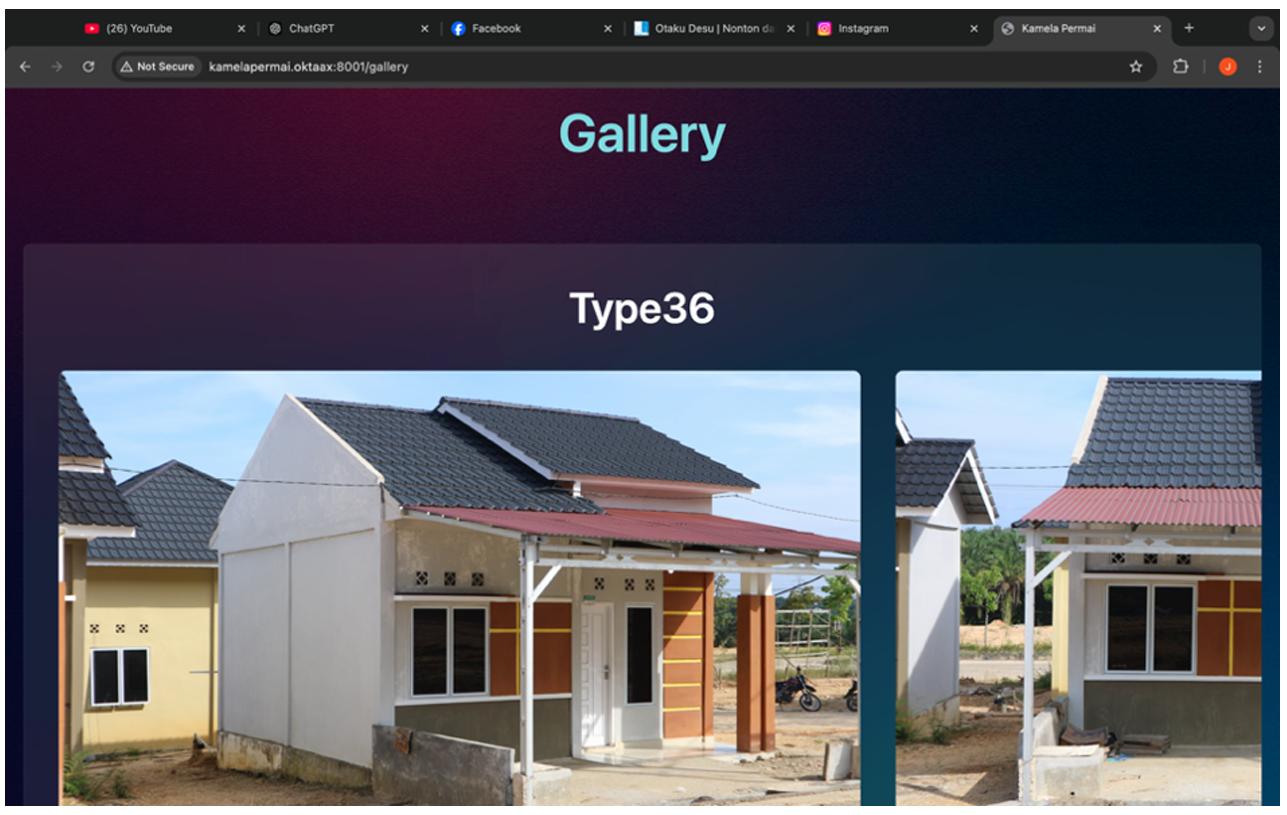
\includegraphics[width=0.75\linewidth]{Implementasi/Gallery.png}
        \caption{Halaman \textit{Gallery}}
    \end{figure}
    
    \item Halaman Panduan
    \par Halaman ini berisi panduan untuk tamu yang ingin booking rumah secara cash atau credit. Halaman dapat dilihat pada gambar berikut.
    \begin{figure}
        \centering
        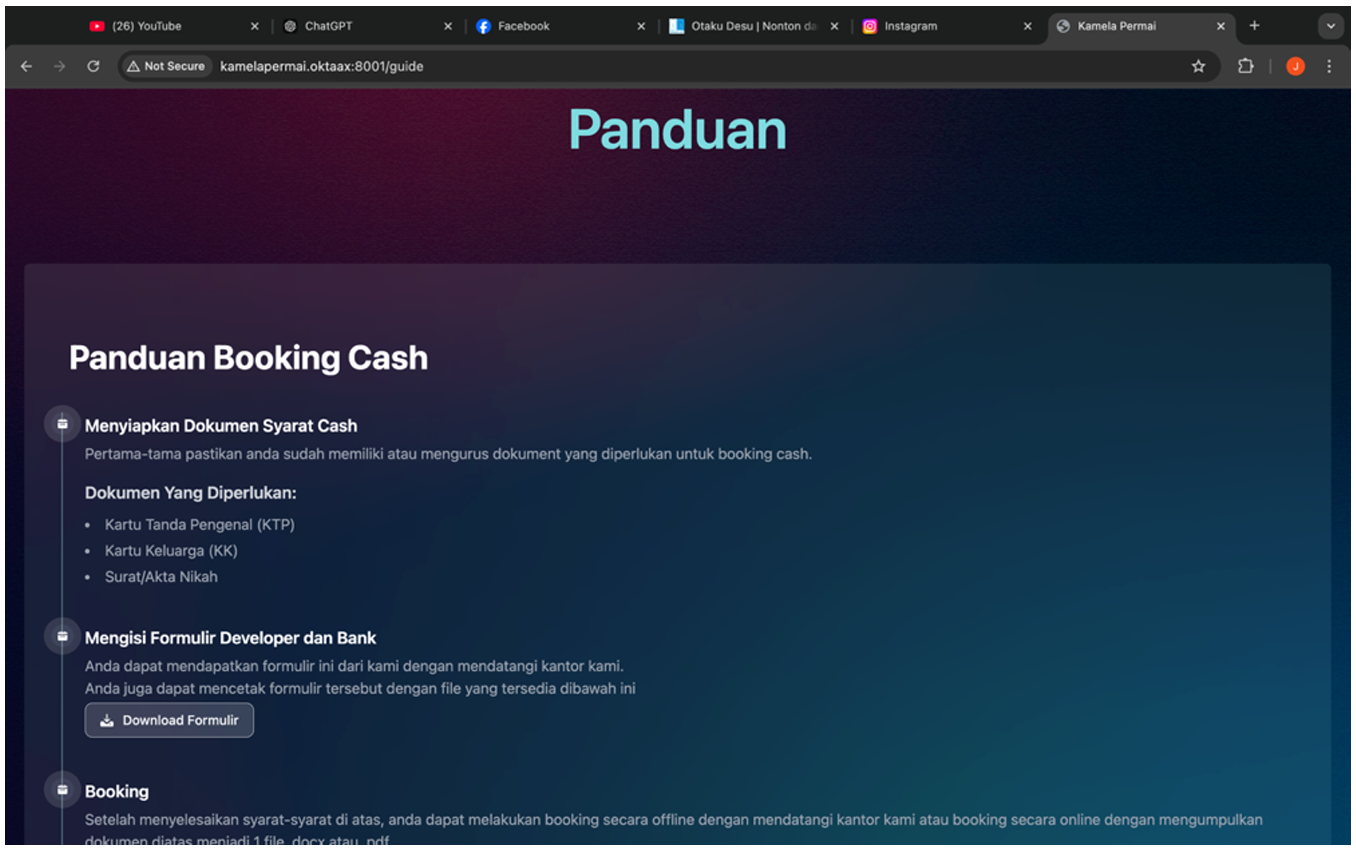
\includegraphics[width=0.75\linewidth]{Implementasi/Panduan.png}
        \caption{Halaman Panduan}
    \end{figure}
    
    \item Halaman \textit{Booking}
    \par Pada halaman ini, tamu yang sudah memilih rumah dapat mengisi form untuk pembookingan. Dapat dilihat pada gambar berikut.
    \begin{figure}
        \centering
        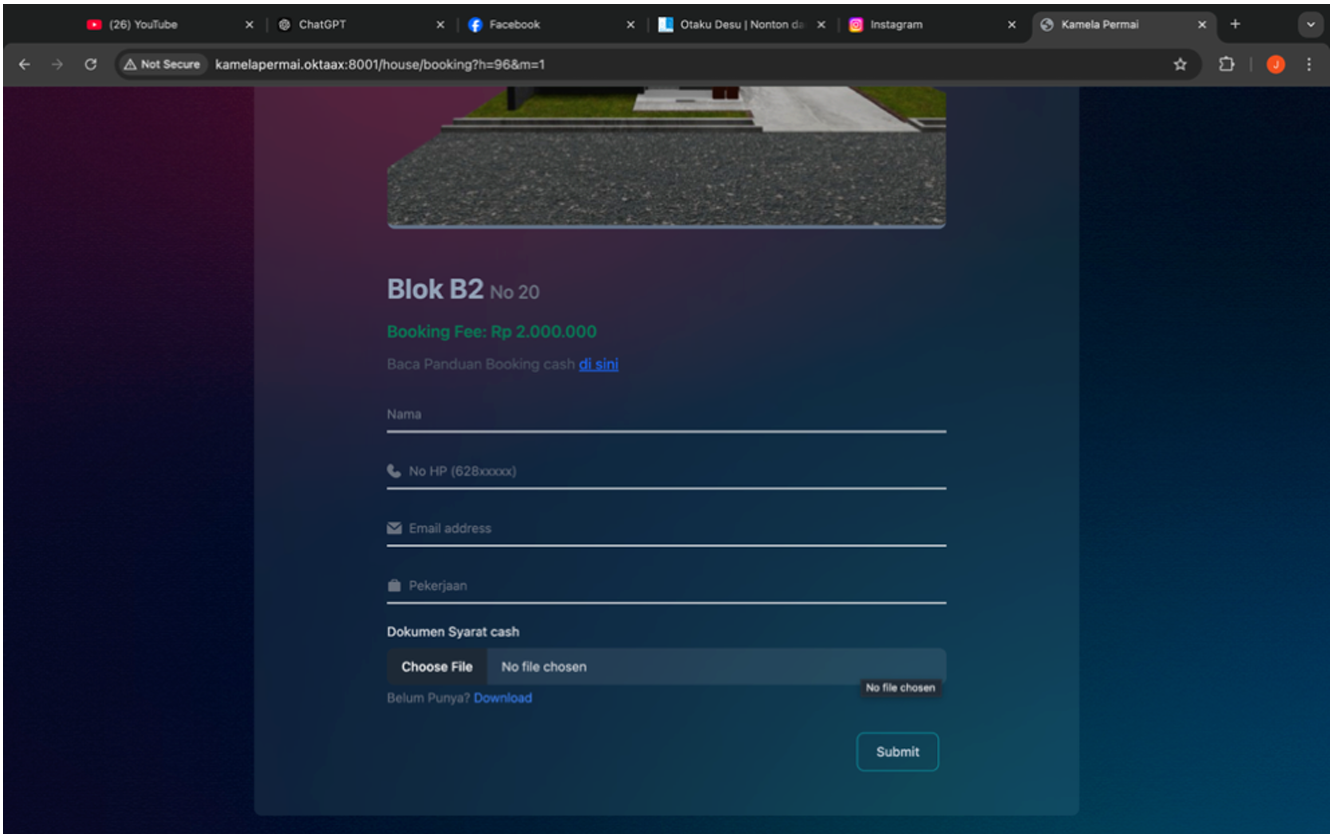
\includegraphics[width=0.75\linewidth]{Implementasi/Booking.png}
        \caption{Halaman \textit{Booking}}
    \end{figure}
    
\end{enumerate}

\subsection{Testing}
\par Dalam pengujian perangkat lunak terdapat berbagai metode yang bisa digunakan untuk melakukan pengujian, misalnya metode \textit{Black Box Testing}. \textit{Black Box Testing} merupakan salah satu metode pengujian yang berfokus pada spesifikasi fungsionalitas dari perangkat lunak. Pengujian ini memberikan gambaran atas sekumpulan kondisi masukan dan melakukan pengujian pada uraian pada fungsional program.
\par \textit{Black Box Testing} digunakan untuk mendeteksi permasalahan berikut:

\begin{enumerate}
\item Fungsi yang salah atau hilang.
\item Kesalahan pada interface.
\item Kesalahan struktur data dan basis data.
\item Kesalahan fungsi.
\item Kesalahan deklrasi dan terminasi.
\end{enumerate}

\par Berikut pengujian yang dilakukan menggunakan \textit{Black Box Testng} pada Sistem Pemesanan Perumahan Kamela Permai:

\renewcommand{\arraystretch}{1.2} % Atur jarak vertikal antar baris
\setlength{\tabcolsep}{4pt} % Atur padding horizontal antar kolom

\begin{scriptsize} % Ukuran teks lebih kecil untuk tabel
\begin{longtable}{|p{2cm}|>{\raggedright}p{4.5cm}|p{4cm}|p{0.8cm}|p{2cm}|}
    \caption{\textit{Black Box Testing}} \label{tab:hasil-pengujian} \\ \hline
    \textbf{Kasus Uji} & \textbf{Prosedur Pengujian} & \textbf{Keluaran yang Diharapkan} & \textbf{Hasil} & \textbf{Kesimpulan} \\ \hline
    \endfirsthead
    \hline
    \endfoot

    % Konten tabel
    Buka sistem & Buka \textit{website} menggunakan \textit{web browser} & Tampilan sistem & \checkmark & Diterima \\ \hline
    Login admin & Masukkan \textit{username} dan \textit{password} lalu klik login & Halaman admin & \checkmark & Diterima \\ \hline
    Booking & 
    - Buka halaman \textit{siteplan} \newline
    - Memilih rumah serta metode \newline
    - Mengisi formulir pemesanan &
    Pemesanan Berhasil & \checkmark & Diterima \\ \hline
    Menu Tamu & Klik tamu & Menu tamu & \checkmark & Diterima \\ \hline
    Menu Rumah & Klik rumah & Menu rumah & \checkmark & Diterima \\ \hline
    Menu \textit{type} & Klik \textit{type} & Menampilkan data \textit{type} & \checkmark & Diterima \\ \hline
    Menu \textit{Logout} & Klik \textit{Logout} & Sesi Berakhir & \checkmark & Diterima \\ \hline

\end{longtable}

\end{scriptsize}

